%\watermark{\fontsize{30pt}{70pt}\selectfont\textcolor{light}{Vertraulich}}

\chapter{Motivation}
\label{cha:Motivation}

Im Fokus der Arbeit steht ein vertikales Supermarktkühlmöbel für Normalkühlung, welches mit Propan (R290) betrieben wird\cite{DINDeutschesInstitutfurNormunge.V..b}. Propan findet vor dem Hintergrund der F-Gas-Verordnung und aufgrund der hohen volumetrischen Kälteleistung immer häufiger Verwendung\cite{EUParlamentRat.2006}\cite{Huber.2016}. Sicherheitsnormen beschränken die maximale Füllmenge eines Kältekreises mit Propan auf \unit{150}{\gram}\cite{DINDeutschesInstitutfurNormunge.V..2014b}. Das AHT-Kühlmöbel für dessen Produktion die Firma Emerson Scrollverdichter liefert ist nicht in der Lage die Zieltemperatur, die zwischen \unit{-1}{\celsius} und \unit{5}{\celsius} liegt, über die gesamte Warenausstellfläche gleichmäßig zu erreichen. Um Gründe für die unzureichende Produktkühlung zu finden und um die Kälteleistung der Kältekreise zu erhöhen werden Untersuchungen in einer Klimakammer durchgeführt. Das Ziel dieser Untersuchungen ist die Identifikation eines optimalen Betriebspunkts durch Zusammenstellung von Komponenten und Maßnahmen, die im Rahmen der durchgeführten Untersuchungen als leistungssteigernd identifiziert wurden, so dass eine ganzheitliche Lösung bestimmt werden kann. 
Vorausgehende Arbeiten umfassen die Installation von Temperatur- und Drucksensoren am Kältekreis und an den Produktdummys um das Verhalten des Systems erfassen und analysieren zu können sowie den Einbau eines kleineren Plattenwärmeübertragers als Verflüssiger. Letzteres zielt auf eine Reduzierung des internen Volumens der Kältekreise um den Mangel an Kältemittel zu kompensieren. Zudem wurden zur genaueren Regelung der Überhitzung thermische durch elektronische Expansionsventile ersetzt. Eine weitere durchgeführte Veränderung ist der Wechsel eines Glykol-Wasser-Gemischs zu Wasser als Wärmetransportmedium für die Verflüssiger.
Die vorausgehenden Arbeiten bezeichnen die Generationen 1 und 2 des Kühlmöbels.
Generation 3 umfasst die im Rahmen der Bachelorarbeit durchgeführten Untersuchungen und Umbauten.
Dabei werden folgende Untersuchungen durchgeführt:

\begin{itemize} 
\item Betrieb mit dem Verdichter ZB09KAU-TFD als Standard- und als Hybridausführung
\item Betrieb mit den Esterölen 3MAF und HATCOL 4467
\item Anpassung der Länge der Abtauintervalle
\item Änderung der Verschaltung der Verdampferpässe
\end{itemize}

Um die Leistung des Verdampfers in einer anderen Verschaltung versuchsunabhängig zu ermitteln wird mithilfe einer geeigneten Software ein Simulationsmodell entwickelt und anschließend anhand der durchgeführten Untersuchungen validiert.

Quellen:
ECODESIGN
EN1127


\chapter{Technik/Methoden}
\label{cha:Technik}

\section{Stand der Technik}
\label{sec:Stand der Technik}

\subsection{Propan in Kälteanlagen}
\label{subsec:Propan in Kälteanlagen}

Der Kohlenwasserstoff Propan (R290) bietet eine umweltfreundliche Alternative zu Kältemitteln wie R22 oder R407c. Propan ist ein natürliches Kältemittel und besitzt eine sehr hohe Verdampfungsenthalpie. Bei gleicher Kälteleistung sind viel geringere Massenströme nötig. Dies resultiert in einem geringerem Energieverbrauch und damit einer hohen Anlageneffizienz.
Es ist mit einem GWP von 0 weder ozonschädlich noch gesundheitsschädlich. Die Verwendung von Propan benötigt aber wegen hoher Entflammbarkeit ein umfassendes Sicherheitkonzept für den Fall von Leckagen\cite{BitzerKuhlmaschinenGmbH.2014}\cite{Huber.2011}.
Um steckerfertige Kühlmöbel ohne spezielle Sicherheitsvorkehrungen betreiben zu können ist die maximale Füllmenge auf \unit{150}{\gram} pro Kältekreis beschränkt.



\subsection{Komponenten einer Kältekompressionsmaschine}
\label{subsec:Komponenten einer Kältekompressionsmaschine}

\subsubsection{Verdichter}
\label{subsubsec:Verdichter}

Mithilfe des Verdichters wird gasförmiges Kältemittel auf ein hohes Druck- und Temperaturniveau verdichtet. Um Kältemittel zu komprimieren finden verschiedene Bauformen Anwendung. Scrollkompressoren zeichnen sich durch hohe Effizienz aus. Diese verfügen über eine sich auf einer kreisförmigen Bahn bewegenden Spirale. Diese Bahn wird durch eine stationäre Spirale verbunden. Durch das bei Rotation zur Spiralmitte kleiner werdende Volumen findet die Verdichtung statt.


\subsubsection{Verflüssiger}
\label{subsubsec:Verflüssiger}

Im Verflüssiger wird gasförmiges, überhitztes Kältemittel durch Wärmeabgabe an ein anderes Fluid enthitzt, verflüssigt und idealerweise unterkühlt. Neben den klassischen Luft-Kältemittel-Wärmeübertragern finden oft Luft-Wasser-Wärmeübertragers Anwendung. Diese Plattenwärmeübertrager ermöglichen aufgrund der höheren Wärmekapazität von Wasser bzw. Sole gegenüber Luft kleineren Bauraum bei gleicher Leistung.

\subsubsection{Expansionsventil}
\label{subsubsec:Expansionsventil}


Im Expansionsventil wird der Druck des Kältemittels nach dem Verflüssiger auf ein niedriges Druckniveau gedrosselt. Dies hat ein Absinken der Sättigungstemperatur zur Folge. Die Enthalpie des Kältemittels bleibt dabei konstant. Durch die bei niedrigerem Druck größer werdende Verdampfungsenthalpie hat das Kältemittel nach der Drosselung einen größeren Dampfanteil als vor dem Ventil. Zum Schutz des Expansionsventiles und um ein fehlerfreies Regelverhalten zu garantieren ist es nötig das Kältemittel vor dem Ventil vollständig zu verflüssigen und zu unterkühlen. Gleichzeitig hat das Expansionsventil die Aufgabe die Überhitzung des Kältemittels auf einen vorgegebenen Wert zu regeln und konstant zu halten. Die Temperatur am Austritt des Verdampfers wird durch einen Temperatursensor an der Saugleitung erfasst. Um das Regelverhalten zu verbessern haben diverse Ventile einen zusätzlichen Drucksensor in der Saugleitung. Dadurch wird eine Verfälschung der Überhitzungsregelung durch Druckabfall über den Verdampfer eliminiert. Elektronische Expansionsventile ermöglichen ein sehr präzises und schnelle Regelverhalten. 

\subsubsection{Verdampfer}
\label{subsubsec:Verdampfer}

Im Verdampfer nimmt das Kältemittel bei niedrigem Druck und entsprechend niedriger Sättigungstemperatur die Wärme des zu kühlenden Fluids auf und verdampft dabei. Die Verdampfungstemperatur soll dabei etwa \unit{10}{\kelvin} unter der Zielprodukttemperatur liegen. In steckerfertigen Kühlmöbeln finden ausschließlich Luft-Kältemittel-Wärmeübertrager Anwendung. Um die wärmeübertragende Fläche zu vergrößern sind die Verdampferrohre mit Lamellen aus Aluminium bestückt. Diese haben für den Einsatzbereich der Normalkühlung Abstände von \unit{4}{\milli\metre} bis \unit{5}{\milli\metre}. Damit verhindert wird, dass flüssiges Kältemittel den Verdichter schädigt wird das Kältemittel um etwa \unit{8}{\kelvin} überhitzt.




\subsection{Kältemittelöle}
\label{subsec:Kältemittelöle}

Öl in Kälteanlagen hat mehrere Aufgaben.
Zur Sicherstellung der Funktionalität des Verdichters ist eine Ölmindestfüllmenge erforderlich. Die Hauptaufgabe des Öles ist eine ausreichende Schmierung des Verdichters, damit der Verschleiß der sich bewegenden Komponenten auf ein Minimum reduziert wird.  Während des Betriebs dissipiert aufgrund von Reibung Wärme, welche an Kältemittel, Öl und über das Gehäuse an die Umgebung abgegeben wird. \newline
Die zweite Aufgabe des Öles ist die Motorkühlung. Das Öl wird damit nur im Verdichter einer Kälteanlage benötigt. Es ist bedingt durch die Bauform des Verdichters nicht möglich den Mittransport eines Teils des Öles in den Kältekreis zu verhindern. Öl erfüllt nur im Verdichter den Zweck seiner Verwendung. In den Wärmeübertragern herrschen andere Drücke und Temperaturen als im Verdichter, was sich auf die physikalischen Eigenschaften des Öles auswirkt. Dort ist die Löslichkeit des Kältemittels im Öl höher, d.h. das Öl ist in der Lage mehr Kältemittel aufzunehmen und dadurch die nutzbare Kältemittelfüllmenge zu reduzieren. \newline
In Kälteanlagen eingesetzte Öle sind Mineralöle und Esteröle. Die im Rahmen der Arbeit untersuchten Öle HATCOL 4467 und 3MAF sind Esteröle, d.h. sie wurden eigens für die Anwendung in einer Kälteanlage synthetisiert\cite{ChemturaCorporation.2017}\cite{LubrizolCorporation.2015}. 
Die in diesem Abschnitt vorgestellten Gleichungen erlauben, unter Berücksichtigung der  Temperaturen und Drücke in den untersuchten Komponenten des Kältekreises, eine Berechnung der Öldichte und dessen kinematischer Viskosität, sowie der Löslichkeit des Kältemittels im jeweiligen Öl. Die Berechnungen dienen dem Vergleich beider Öle hinsichtlich der  Erhöhung der Kälteleistung. In den folgenden Gleichungen bezeichnet $T$ die Temperatur des Öles in $Kelvin$ und $p$ den Druck in der jeweiligen Komponente in $\bbar$. Die Koeffizienten $a_1$ bis $a_9$ sind je nach Öl und Gleichung verschieden.

Die Öldichte $\rho$ in $\frac{\kilo\gram}{\cubic\metre}$ ergibt sich gemäß Gleichung~\ref{eq:1}: 

\begin{equation}
\label{eq:1}
\rho = a_{1} + a_{2}T + a_{3}T^2 + \omega(a_{4}+ a_{5}T + a_{6}T^2) + \omega^2(a_{7}+ a_{8}T + a_{9}T^2)
\end{equation}

Die Berechnung der kinematische Viskosität $\nu$ in $cSt$ erfolgt gemäß Gleichung~\ref{eq:3}:

\begin{align}
\label{eq:3}
	\begin{split}
		\ln(\ln(\nu + 0.7 + e^{-\nu} K_{0} (\nu + 1.244068))) =~ 
		&a_{1} + a_{2}\ln{T} + 	a_{3}\ln^2{T} \\
		&+ \omega(a_{4} + a_{5}\ln{T} + a_{6}\ln^2{T}) \\
		&+ \omega^2(a_{7} + a_{8}\ln{T} + a_{9}\ln^2{T}) 
	\end{split}
\end{align}

mit der Hilfsgröße $K_0$ gemäß Gleichung~\ref{eq:3_1}:

\begin{equation}
\label{eq:3_1}
K_0 = BesselK(\nu + 1.244068 , 0)
\end{equation}

Gleichung~\ref{eq:2} ermöglicht eine Berechnung der Löslichkeit des Kältemittels $\omega$ in $\frac{\gram KM}{\gram Öl}$. 

\begin{equation}
\label{eq:2}
\log(p) = a_{1} + \frac{a_{2}}{T} + \frac{a_{3}}{T^2} + \log(\omega)( a_{4} + \frac{a_{5}}{T} + \frac{a_{6}}{T^2}) + \log^2(\omega)( a_{7} + \frac{a_{8}}{T} + \frac{a_{9}}{T^2})
\end{equation}

Eine iterative Berechnung liefert eine Lösung für das Gleichungssystem.







\section{Das Kühlregal}
\label{sec:Das Kühlregal}

Der Mittelpunkt der durchgeführten Untersuchungen ist ein vertikales Verkaufskühlmöbel der Firma AHT.
Es umfasst auf einer Länge von \unit{3,75}{\metre} vier Regalböden um Produkte zu kühlen und auszustellen. Ein von oben herabfallender Luftschleier ermöglicht ein türloses Design des Regals. Ein Nachtbetrieb mit geschlossener Jalousie ist möglich. Die Kälteerzeugung wird, wie in Abbildung~\ref{fig:IDC150} ersichtlich, durch drei seperate Kältekreisläufe gewährleistet. Das verwendete Kältemittel ist Propan (R290). Jeder Kreis besitzt eine Kältemittelfüllmenge von \unit{150}{\gram} und eine Ölfüllmenge von \unit{470}{\gram}. Um die Kältemittelfüllmenge zu reduzieren wurden bereits vor Beginn der Untersuchungen kältetechnische Komponenten mit geringerem internen Volumen eingebaut. Die Verdichter sind Scrollkompressoren der Firma Emerson.  Im Rahmen der Untersuchungen finden zwei Ausführungen desselben Verdichtermodells Anwendung. Das von Emerson gefertigte Modell ZB09KAU-TFD in Hybridausführung besitzt eine Motorwicklung aus Aluminium. Dasselbe Modell in Standardausführung besitzt eine Kupferwicklung. Drei Plattenwärmeübertrager der Firma SWEP dienen als Verflüssiger. Sie besitzen je 20 Platten und eine Nennleistung von je \unit{2,7}{\kilo\watt}. Die Expansionsventile der Firma Alco sind elektronisch regelbar und besitzen einen Temperatur- sowie Drucksensor in der Saugleitung. Die drei Kreisläufe durchlaufen mit je sechs Durchgängen einen gemeinsamen Verdampfer dessen Lamellenabstand \unit{5}{\milli\metre} beträgt. Sechs Lüftermotoren der Firma EBM Pabst befördern die Luft mit einer konstanten Drehzahl von \unit{1400}{U\per\min} durch den Verdampfer.

\begin{figure} %[!htb]
\centering
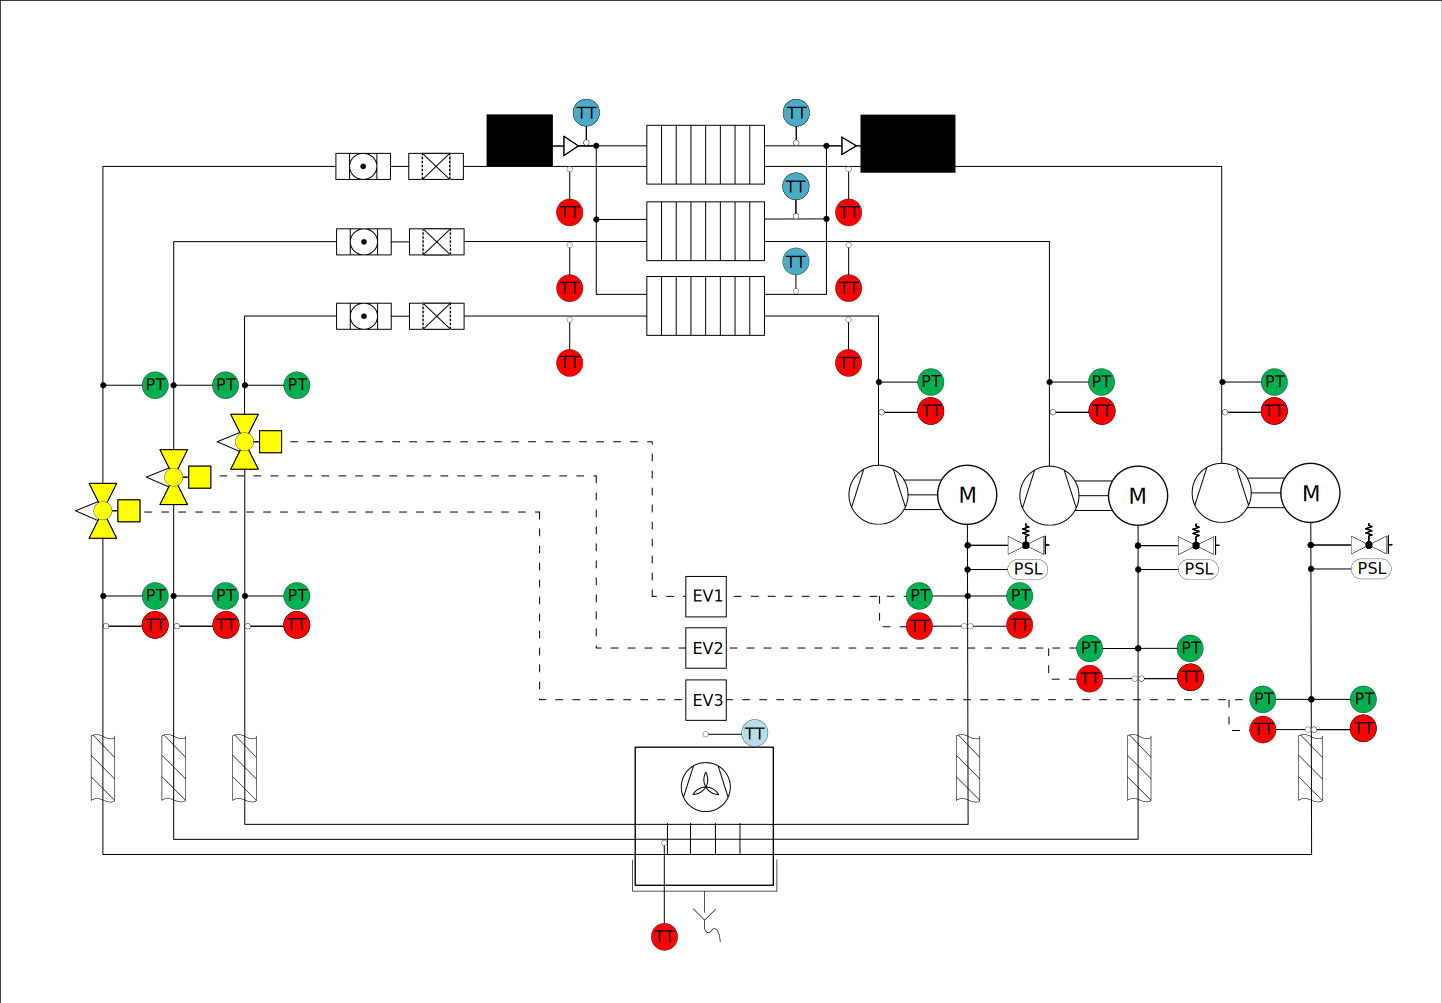
\includegraphics[scale=.5,angle=90]{Pictures/IDC150.pdf}
\caption{Kältekreise des Kühlmöbels}
\label{fig:IDC150}
\end{figure}


\section{Die Klimakammer}
\label{sec:Die Klimakammer}

Um während den Untersuchungen gleichbleibende Umgebungsbedingungen zu generieren und  reproduzierbare Ergebnisse zu erzielen, wird das Kühlregal in einer Klimakammer betrieben.
Wie in Abbildung~\ref{fig:Klimakammer} zu erkennen besteht die Klimakammer aus zwei kleineren Kammern mit eigenständigen Zuluftregelungen. Aufgrund der Größe des Regals wurde die Trennwand zwischen den Kammern entfernt. Die Zuluftaufbereitung übernimmt dabei die Klimaanlage der Kammer B. Damit die aufbereitete Luft den Raum über dessen gesamte Länge durchströmt wurde die Ansaugöffnung von Kammer B mit einer Decke, die bis zum Ende des Raums reicht, abgedeckt. Vor den Luftauslassgittern besitzen die Kammern Umlenkbleche. Diese sollen eine gleichmäßige Verteilung des Luftmassenstroms über den Austrittquerschnitt erzielen. Die Klimaanlagen sind in der Lage die angesaugte Raumluft zu kühlen, aufzuheizen sowie zu be- und entfeuchten. Die Regelung findet dabei über einen Computer statt. Mithilfe des Programms LabView, welches eine intuitive Benutzeroberfläche bietet, lässt sich Einfluss auf die Soll-Werte, die Dauer der jeweiligen Untersuchung und die Einstellung der Regelparameter nehmen. 
Jede Kammer besitzt zudem einen Wasseranschluss dessen Vorlauftemperatur regulierbar ist.
Die Verflüssiger des Kühlregals werden mit temperiertem Wasser der Regelung von Kammer A beaufschlagt. Die Regelung der Verflüssigungstemperatur geschieht mittels zwei Pumpen in einem primären und einem sekundären Wasserkreislauf. Die Pumpe im primären Wasserkreislauf beaufschlagt die Verflüssiger mit Wasser und hält eine Temperaturdifferenz von \unit{5}{\kelvin} über diesen konstant. Die Pumpe des sekundären Wasserkreislaufs regelt über einen Wärmeübertrager zwischen den beiden Kreisen die Temperatur des Wassers am Eintritt des Verflüssigers auf \unit{35}{\celsius}.


\begin{figure}[htb]
\centering
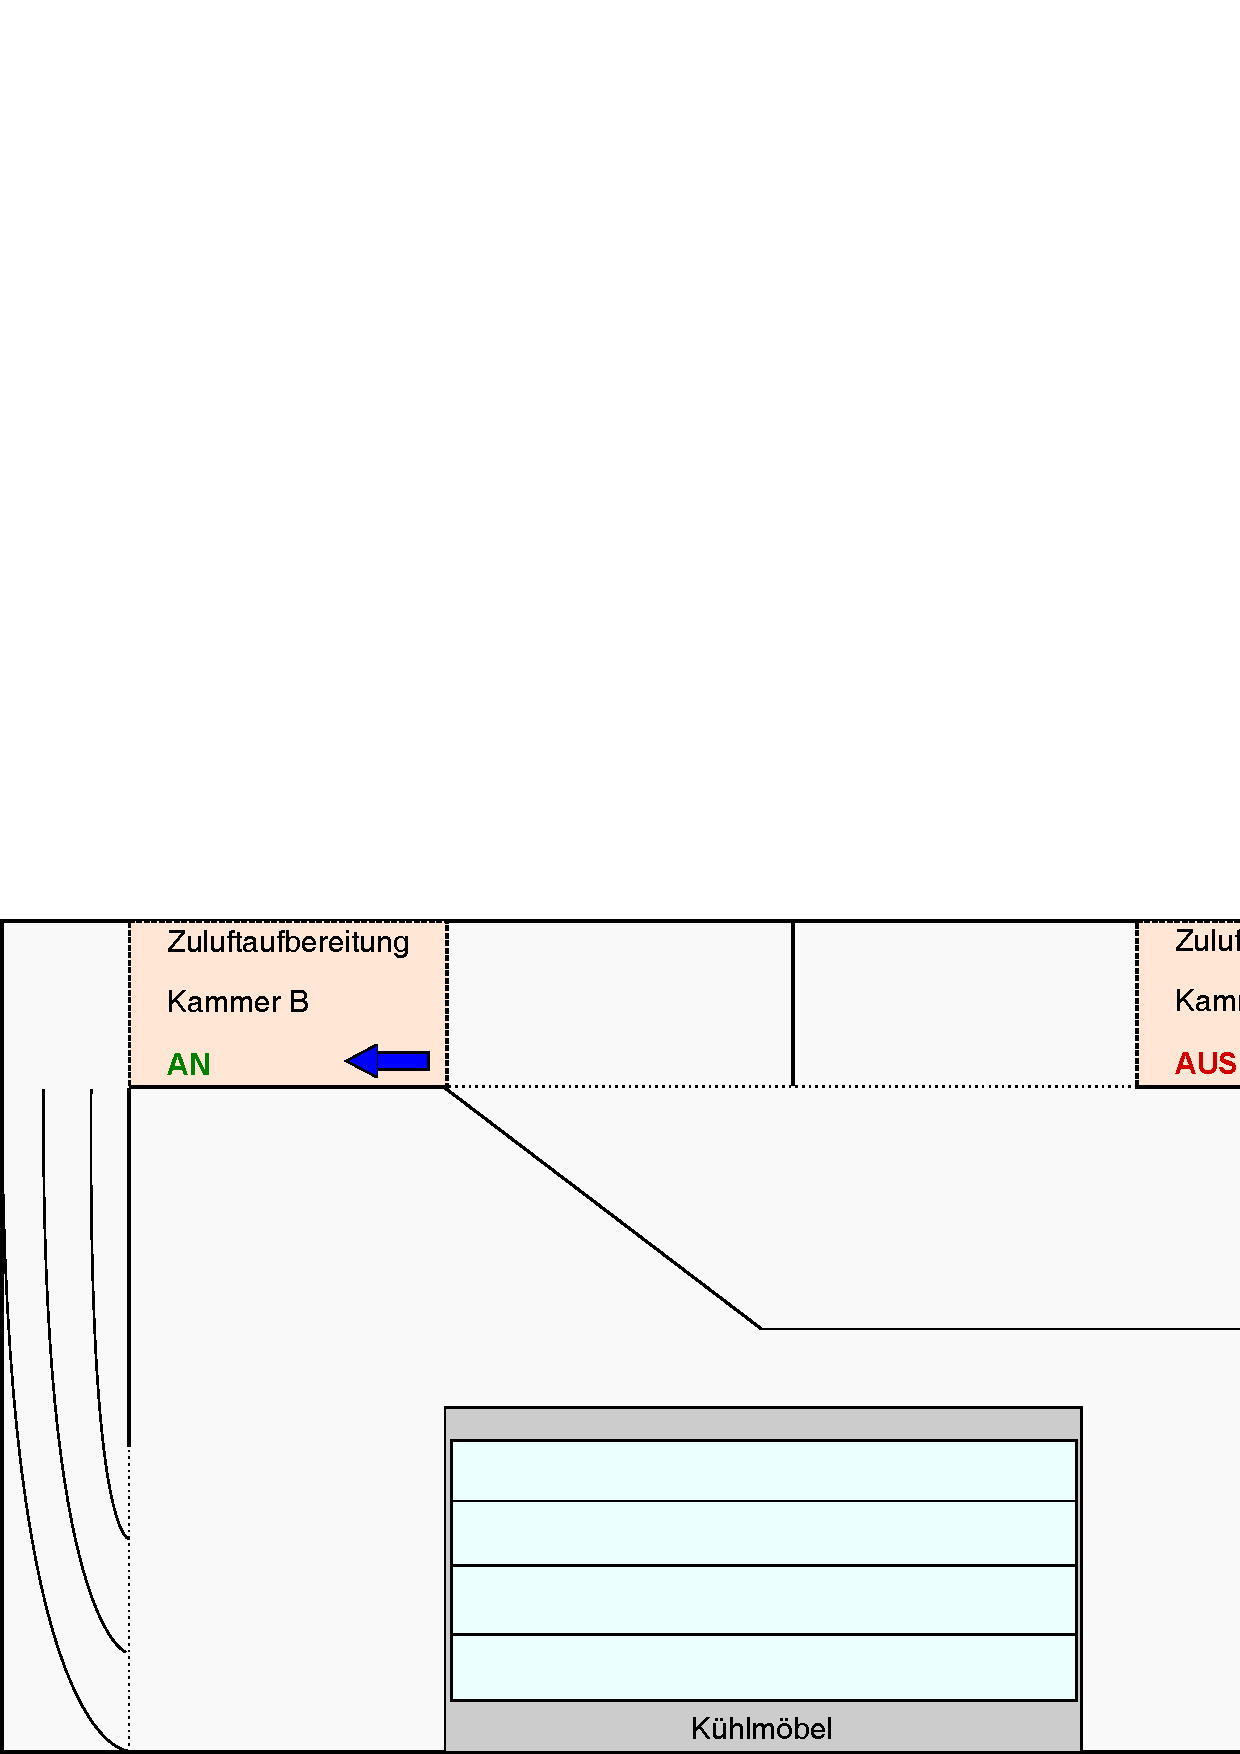
\includegraphics[scale=.6]{Pictures/ClimateChamber.pdf}
\caption{Klimakammer}
\label{fig:Klimakammer}
\end{figure}

\section{Messdaten und Berechnungsgrößen}
\label{sec:Erfassung von Messdaten}

Es werden Geräte und Programme verwendet um alle physikalischen Größen während des Betriebs möglichst genau zu erfassen und zu speichern. Insgesamt finden drei Systeme Anwendung um sensorbasiert Daten zu erfassen, umzuwandeln und in Tabellenform zu speichern. Alle erfassten sowie berechneten Messdaten werden über die letzten \unit{75}{\%} des letzten Kühlzyklus in einem Untersuchungszeitraum von \unit{24}{\hour} gemittelt. Dies dient der Vergleichbarkeit.

\subsection{Messdaten der Klimakammer}
\label{subsec:Messdaten der Klimakammer}

Die in Abschnitt~\ref{sec:Die Klimakammer} vorgestellte Klimakammer wird über LabView gesteuert. Die erfassten Messdaten sind raumluftseitig Ist- und Mittelwerte der Temperaturen sowie die relative Luftfeuchtigkeit. Wasserseitig werden Wassermassenstrom sowie Vor- und Rücklauftemperatur gemessen. 
Die Sensoren, welche die Regelgrößen Temperatur und relative Luftfeuchtigkeit aufnehmen, sind zuluftseitig in der Nähe des Auslassgitters positioniert. Alle Temperatursensoren besitzen eine Messungenauigkeit von $\pm$~\unit{1}{\kelvin}. Die Regelgröße der Temperatur entspricht dem Mittelwert von drei, über die Höhe des Luftauslassgitters verteilten Temperatursensoren. Wird der Betrieb der Klimakammer über das Programm gestartet so wird eine Exceldatei erstellt in die in einem Intervall von \unit{1}{\second} die erfassten Daten geschrieben werden.


\subsection{Messdaten des Kühlregals}
\label{subsec:Messdaten der Klimakammer}

Mithilfe des Programms NI SignalExpress werden die Messdaten des Kühlregals und der Kältekreisläufe via Modbus erfasst. Um die Temperaturen zu messen werden Thermoelemente  und um die Drücke zu messen Hochgenauigkeitsdruckaufnehmer verwendet. Die erfassten Messwerte sind die Produkttemperaturen sowie Ein- und Austrittstemperatur der Luft am Verdampfer des Kühlregals, die Temperaturen an verschiedenen Positionen der Kältekreisläufe und die Relativdrücke des Kältemittels im System in Heißgasleitung, Flüssigkeitsleitung, Einspritzleitung und Saugleitung. Die Positionen der Sensoren an den Kältekreisläufen sind aus Abbildung~\ref{fig:IDC150} ersichtlich. Zudem wurde noch die Temperatur des Kältemittels nach jedem einzelnen Durchgang durch den Verdampfer erfasst.
In einem Intervall von \unit{5}{\second} werden die erfassten Daten in eine Exceltabelle geschrieben. SignalExpress erstellt in Echtzeit Graphen der Messwerte. Somit lässt sich das Verhalten des Systems jederzeit beobachten.

\subsection{Messdaten des Leistungsanalysators}
\label{subsec:Messdaten des Leistungsanalysators}

Um den Zustand des Systems auch elektroseitig zu erfassen wird ein Yokogawa WT3000 Leistungsanalysator verwendet. Dieser ist in der Lage Spannungen, Ströme mit einer Genauigkeit von \unit{0,02}{\%} zu erfassen und daraus Blind-, Wirk- und Scheinleistungen zu berechnen. Die abgenommenen Komponenten sind die einzelnen Verdichter, die Ventilatoren und die restlichen Verbraucher des Kühlregals, wie Licht und Relays.
Das Gerät speichert die erfassten und berechneten Messwerte in Tabellenform auf einem externen Datenspeicher. Die Intevalllänge beträgt hierbei \unit{5}{\second}.


\subsection{Berechnungsgrößen}
\label{subsec:Berechnungsgrössen}

Auf Basis der mithilfe der Messtechnik erfassten Größen werden Leistungen und Bewertungsgrößen berechnet. Diese ermöglichen es, das Verhalten des Systems zu visualisieren und bewerten zu können.
Der an einem Wärmeübertrager übertragene Wärmestrom lässt sich mit Gleichung~\ref{eq:4} allgemein formulieren.

\begin{equation}
\label{eq:4}
\dot{Q}= kA(T_A - T_B) = \dot{M}_{A}(h_{WÜ,aus} - h_{WÜ,ein})
\end{equation}

Die am Verflüssiger übertragene Leistung berechnet sich auf Basis der Temperaturen und des Massenstroms des Wassers nach Gleichung~\ref{eq:5}.

\begin{equation}
\label{eq:5}
\dot{Q}_{cd}= \frac{\dot{M}_{W}}{3} c_{p,W} (T_{W,aus} - T_{W,ein})
\end{equation}

Da unter den Testbedingungen nicht immer eine Unterkühlung des Kältemittels und damit ein Verlassen des Zweiphasengebietes stattfindet, wird die Enthalpie am Verflüssigeraustritt bzw. am Verdampfereintritt mithilfe der erfassten Messdaten am Verflüssigereintritt und der zuvor berechneten Verlüssigerleistung nach Gleichung~\ref{eq:6} berechnet.

\begin{equation}
\label{eq:6}
h_{cd,aus} = h_{cd,ein} - \frac{\dot{Q}_{cd}}{\dot{M}_{KM}}
\end{equation}

Der Kältemittelmassenstrom wird auf Basis der Verdampfungs- und der Verlüssigungstemperatur, sowie vom Hersteller ermittelten Koeffizienten anhand von Gleichung~\ref{eq:7} berechnet.

\begin{align}
\label{eq:7}
	\begin{split}
	\dot{M}_{KM} = &C_0 + C_1*T_{ev,sat} + C_2*T_{cd,sat} + C_3*T_{ev,sat}^2 \\
	&+C_4*T_{ev,sat}*T_{cd,sat} + C_5*T_{cd,sat}^2 + C_6*T_{ev,sat}^3 \\
	&+ C_7*T_{cd,sat}*T_{ev,sat}^2 +C_8*T_{ev,sat}*T_{cd,sat}^2 + C_9*T_{cd,sat}^3
	\end{split}
\end{align}

Somit lässt sich mit Gleichung~\ref{eq:8} die Verdampferleistung bestimmen.

\begin{equation}
\label{eq:8}
\dot{Q}_{ev}= \dot{M}_{KM}(h_{ev,aus} - h_{ev,ein})
\end{equation}


Um die Effizienz des Systems in einem Betriebspunkt zu bewerten wird die EER-Kennzahl mit Gleichung~\ref{eq:9} berechnet, welche den am Verdampfer übertragenen Wärmestrom ins Verhältnis zur aufgenommenen elektrischen Leistung setzt\cite{Muller.2016}:

\begin{equation}
\label{eq:9}
EER = \frac{\dot{Q}_{ev}}{P_{el}}
\end{equation}



\section{Testbedingungen nach Norm}
\label{sec:Testbedingungen nach Norm}

Die Norm DIN EN ISO 23953-2 liefert Vorgaben zum Aufbau des Prüfstandes, zur Position der Messtechnik und zu Berechnungsmethoden. Bei allen Tätigkeiten wurde sich an dieser orientiert um reproduzierbare sowie vergleichbare Ergebnisse zu erzielen. Rahmenbedingung ist, dass alle Untersuchungen, nach Tabelle~\ref{tab:Klimaklassen}, bei Klimaklasse 3 durchgeführt werden. Die erzielten Produkttemperaturen des Kühlmöbels müssen dabei, gemäß Tabelle~\ref{tab:Temperaturklassen}, zwischen \unit{5}{\celsius} und \unit{-1}{\celsius} liegen.
Um Kühlgut möglichst genau zu simulieren, werden je \unit{1}{\kilogram} schwere M-Pakete aus Silikon verwendet.
Diese werden entsprechend Abbildung~\ref{fig:Anordnung der M-Pakete} positioniert und jene die mit einem X gekennzeichnet sind mit Temperatursensoren versehen.
Der Messpunkt für die Temperatur und die relative Luftfeuchte muss mittig der Länge der Kühlmöbels und \unit{300}{\milli\metre} vor dessen Oberkante liegen.
Voraussetzung für eine normgerechte Messung ist zudem, dass eine Bewegung der Luft vorhanden ist. Deren Geschwindigkeit muss an den drei Messpunkten auf der Linie A-A in Abbildung~\ref{fig:Messpunkte} zwischen \unit{0,1}{\meter\per\second} und \unit{0,2}{\meter\per\second} liegen\cite{DINDeutschesInstitutfurNormunge.V..}.

Die erfassten Messwerte und die auf deren Basis berechneten Leistungen sowie Bewertungsgrößen werden über die letzten \unit{75}{\%} des letzten Kühlzyklus in einem Untersuchungszeitraum von \unit{24}{\hour} gemittelt.





% Please add the following required packages to your document preamble:
% \usepackage[table,xcdraw]{xcolor}
% If you use beamer only pass "xcolor=table" option, i.e. \documentclass[xcolor=table]{beamer}
\begin{table}[h!]
\centering
\caption{Klimaklassen.}
\label{tab:Klimaklassen}
\begin{tabular}{|c|c|c|c|c|}
\hline
\textbf{\begin{tabular}[c]{@{}c@{}}Klimaklasse des \\ Prüfraums\end{tabular}} & \textbf{\begin{tabular}[c]{@{}c@{}}Trockenkugel-\\ temperatur\end{tabular}} & \textbf{\begin{tabular}[c]{@{}c@{}}Relative \\ Luftfeuchte\end{tabular}} & \textbf{Taupunkt} & \textbf{\begin{tabular}[c]{@{}c@{}}Wasserdampf-\\ gehalt \\ in trockener Luft\end{tabular}} \\
                                                                              &                                                                             & \%                                                                       & °C                & g/kg                                                                                        \\ \hline
0                                                                             & 20                                                                          & 50                                                                       & 9,3               & 7,3                                                                                         \\ \hline
1                                                                             & 16                                                                          & 80                                                                       & 12,6              & 9,1                                                                                         \\ \hline
8                                                                             & 23,9                                                                        & 55                                                                       & 14,3              & 10,2                                                                                        \\ \hline
2                                                                             & 22                                                                          & 65                                                                       & 15,2              & 10,8                                                                                        \\ \hline
\rowcolor[HTML]{FFFe65}
3                                                                             & 25                                                                          & 60                                                                       & 16,7              & 12                                                                                          
\\ \hline
4                                                                             & 30                                                                          & 55                                                                       & 20                & 14,8                                                                                        \\ \hline
5                                                                             & 27                                                                          & 70                                                                       & 21,1              & 15,8                                                                                        \\ \hline
6                                                                             & 40                                                                          & 40                                                                       & 23,9              & 18,8                                                                                        \\ \hline
7                                                                             & 35                                                                          & 75                                                                       & 30                & 27,3                                                                                        \\ \hline
\end{tabular}
\end{table}

\begin{figure}[h!tb]
\centering
\includegraphics[scale=.12]{Pictures/multi-deck-chilled-cabinet.pdf}
\caption{Anordnung der M-Pakete und der Temperatursensoren.}
\label{fig:Anordnung der M-Pakete}
\end{figure}

% Please add the following required packages to your document preamble:
% \usepackage[table,xcdraw]{xcolor}
% If you use beamer only pass "xcolor=table" option, i.e. \documentclass[xcolor=table]{beamer}
\begin{table}[h!]
\centering
\caption{Temperaturklassen der M-Pakete.}
\label{tab:Temperaturklassen}
\begin{tabular}{|c|c|c|}
\hline
\textbf{Klasse} & \textbf{\begin{tabular}[c]{@{}c@{}}Höchste Temperatur,\\ des wärmsten\\ M-Pakets gleich oder\\ niedriger als\end{tabular}} & \textbf{\begin{tabular}[c]{@{}c@{}}Niedrigste Temperatur,\\ des kältesten\\ M-Pakets gleich oder\\ höher als\end{tabular}} \\ \cline{2-3} 
                & \multicolumn{2}{c|}{°C}                                                                                                                                                                                                                                 \\ \hline
L1              & -15                                                                                                                        & -                                                                                                                          \\ \hline
L2              & -12                                                                                                                        & -                                                                                                                          \\ \hline
L3              & -12                                                                                                                        & -                                                                                                                          \\ \hline
\rowcolor[HTML]{FFFE65} 
M1              & +5                                                                                                                         & -1                                                                                                                         \\ \hline
M2              & +7                                                                                                                         & -1                                                                                                                         \\ \hline
H1              & +10                                                                                                                        & +1                                                                                                                         \\ \hline
H2              & +10                                                                                                                        & -1                                                                                                                         \\ \hline
S               & \multicolumn{2}{c|}{Sonderklasse}                                                                                                                                                                                                                       \\ \hline
\end{tabular}
\end{table}




\begin{figure}[h!tb]
\centering
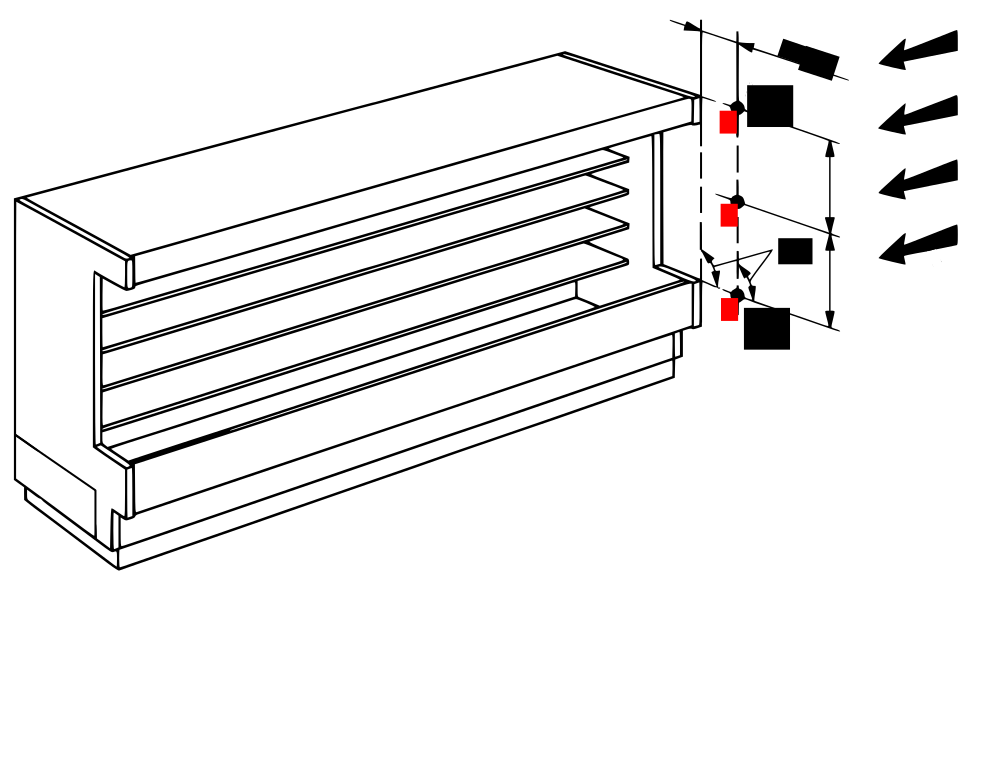
\includegraphics[scale=.5]{Pictures/idc_meas2.pdf}
\caption{Messpunkte.}
\label{fig:Messpunkte}
\end{figure}


\section{Simulationsmodell für Verschaltung der Verdampferrohre}
\label{sec:Simulationsmodell}

Mithilfe des Programms EES (Engineering Equation Solver) wurde im Rahmen der Untersuchungen ein Modell erstellt, welches es ermöglicht den Effekt einer anderen Verschaltung der kältemittelführenden Leitungen innerhalb des Verdampfers auf dessen Kälteleistung zu simulieren. Grundidee hinter dem Modell ist den, durch den hohen Kältemittelmassenstrom bei gleichzeitig geringem Durchmesser der Verdampferrohre bedingten, Druckabfall und das damit einhergehende Absinken der Sättigungstemperatur zur Erhöhung der Kälteleistung zu nutzen. Im Ausgangsmodell durchströmt das Kältemittel den Verdampfer im Gegenstromprinzip. Aufgrund des Druckabfalls verhält sich diese Anordung wie eine Kombination aus Gleich- und Gegenstrom. Wird nun die Anordnung der Rohre dahingehend geändert, dass das Kältemittel den Verdampfer von dessen Mitte aus im Gleichstrom mit der Luft nach oben durchströmt, aber die überhitzten Rohrreihen noch immer beim Lufteintritt sind, so erzielt man den gegenteiligen Effekt: Der Wärmeübertrager bietet eine Kombination aus Gleich- und Gegenstrom, verhält sich aber wie ein reiner Gegenstromverdampfer. Hierbei ist am Verdampferaustritt der Luft eine höhere Temperaturdifferenz zum Kältemittel zu erwarten. Den Vergleich zeigt Abbildung~\ref{fig:Vergleich der Verdampferschaltungen}.
Das Modell soll zeigen ob diese Maßnahme einen bedeutenden Effekt erzielen kann und wird anschließend im Versuch validiert.


\begin{figure}[htb]
\centering
	\subfigure[Ausgangsschaltung]{\includegraphics[scale=0.4]{Pictures/Verdampfer_Gegenstrom.pdf}}
	\subfigure[veränderte Schaltung]{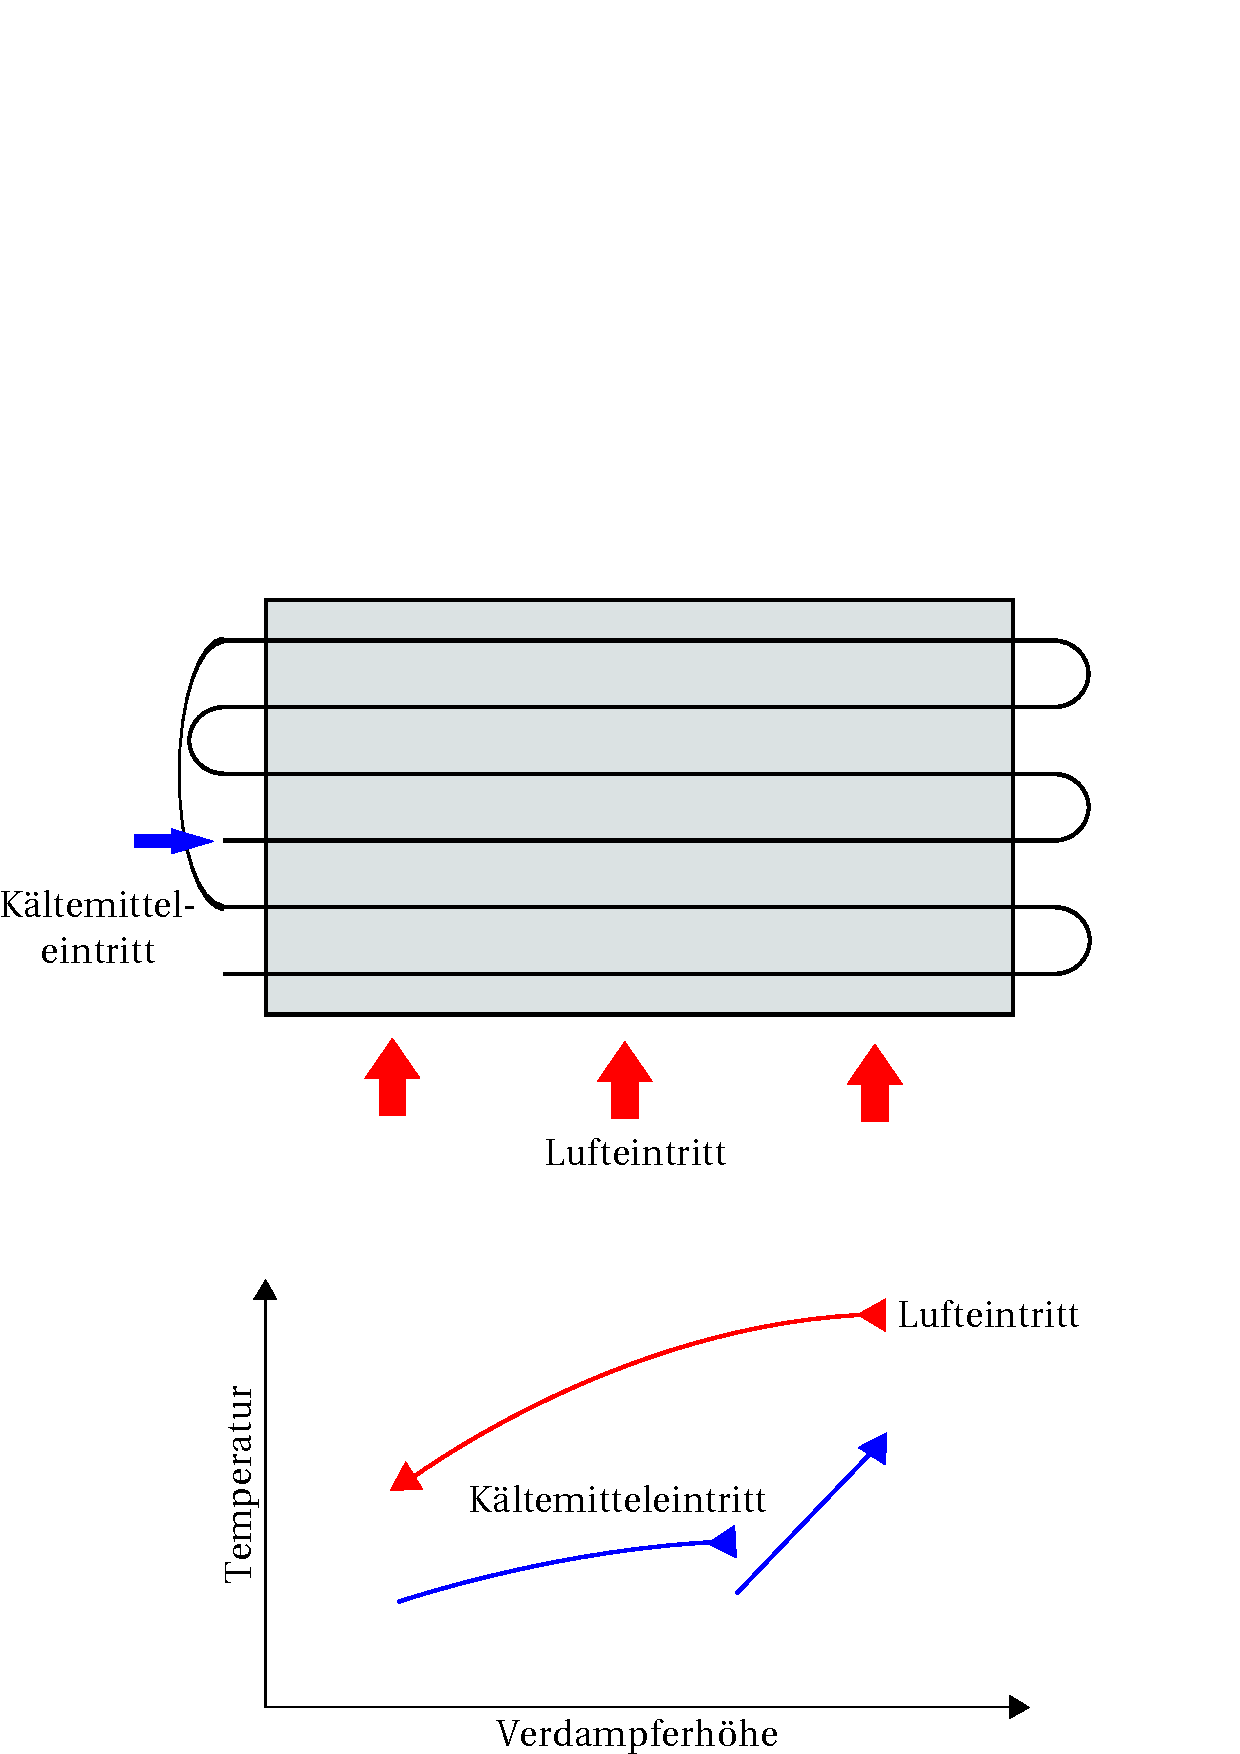
\includegraphics[scale=0.4]{Pictures/Verdampfer_Gleich-Gegenstrom.pdf}}
\caption{Vergleich der Verdampferschaltungen.}
\label{fig:Vergleich der Verdampferschaltungen}
\end{figure}


\subsection{Modellierung mit EES}
\label{subsec:Modellierung mit EES}

EES ist ein Gleichungslöser, der es erlaubt Gleichungen mit Unbekannten unabhängig ihrer Reihenfolge effizient zu lösen. Zudem besitzt EES eine Vielfalt integrierter mathematischer, sowie thermodynamischer und physikalischer Funktionen auf die sich bequem zugreifen lässt\cite{Klein.2000}. Ausschlaggebend für den Entscheid über die Nutzung des Programms ist vorallem die integrierte Stoffdatenbank, welche den Zugriff auf die Daten einer Vielzahl von idealen sowie realen Fluiden erlaubt. Eine objektorientierte Modellierung ist leider nicht ohne Weiteres möglich, wodurch der Entwicklungsaufwand stark erhöht wird. Damit das Programm genaue Ergebnisse liefert ist es nötig, physikalisch sinnvolle und und möglichst genaue Begrenzungen der erstellten Variablen anzugeben. 
Weitere Programmfunktionen erlauben die Erstellung einer Benutzeroberfläche sowie die Erstellung von Tabellen und Graphen. Als sehr nützlich erweist sich dabei die Möglichkeit Stoff-Eigenschaftsdiagramme wie z.B. Mollier- oder log-p-h-Diagramme zu erstellen.



\subsection{Berechnung des Druckabfalls in der Zweiphasen-Strömung}
\label{subsec:Berechnung des Druckabfalls in der Zweiphasen-Strömung}

Die Ausgangsberechnung auf der alle weiteren Berechnung basieren, ist die des Druckabfalls innerhalb der Kältemittelströmung.
Der gesamte Druckabfall setzt sich aus einem Reibungsanteil, einem Beschleunigungsanteil und einem statischen Anteil zusammen\cite{SpringerVerlagGmbH.2013}:

\begin{equation}
\label{eq:10}
\Delta p =  \Delta p_{Reibung} \pm \Delta p_{statisch} \pm \Delta p_{Beschleunigung}
\end{equation}

Der statische Anteil, sowie der Beschleunigungsanteil sind von einer viel kleineren Dimension und werden deshalb als vernachlässigbar angenommen. Um den durch Reibung bedingten Druckabfall zu berechnen muss zunächst bestimmt werden ob die Gasphase dispers oder kontinuierlich ist, d.h. ob Gasblasen getrennt und verteilt in der Flüssigkeit transportiert werden oder zusammenhängend strömen.

\begin{equation}
\label{eq:11}
\Delta p_{Reibung} = \int_{l_1}^{l_2} \left( \frac{dp}{dl} \right)_{Reibung} dl
\end{equation}


Die Gasphase ist dispers, wenn gilt:

\begin{equation}
\label{eq:12}
\frac{1}{\beta} = \frac{\dot{V_G}}{\dot{V_F}} = \frac{x\rho_F}{(1-\dot{x})\rho_D} \leq \frac{12\sqrt{Fr}}{1+\frac{\sqrt{Fr}}{7}}
\end{equation}

und als kontinuierlich, wenn gilt:

\begin{equation}
\label{eq:13}
\frac{1}{\beta} = \frac{\dot{V_G}}{\dot{V_F}} = \frac{x\rho_F}{(1-\dot{x})\rho_D} > \frac{12\sqrt{Fr}}{1+\frac{\sqrt{Fr}}{7}}
\end{equation}

In allen durchgeführten Berechnungen ist die Dampfphase als kontinuierlich zu betrachten, daher wird sich im Rahmen dieser Ausführungen auf die Gleichungen dieser Annahme beschränkt. Der Reibungsdruckabfall wird wesentlich durch einen intensiven Impulsaustausch zwischen den beiden Phasen beeinflusst. In den Gleichungen wird die Zweiphasenströmung wie eine Dampfströmung behandelt und der Einfluss der flüssigen Phase durch eine Korrekturgröße $\gamma$ berücksichtigt:

\begin{equation}
\label{eq:14}
\left( \frac{dp}{dl} \right)_{Reibung} = \xi_D \frac{\dot{m}^2 x^2}{4\rho_D} \left(\frac{1}{1-\gamma} \right)^2
\end{equation}

Dabei ist $\xi_D$ der Reibungsbeiwert:

\begin{equation}
\label{eq:15}
\frac{1}{\xi_D} = 2\log(Re_D \sqrt{\xi_D})-0.8
\end{equation}

mit der Reynoldszahl der dampfförmigen Phase:

\begin{equation}
\label{eq:16}
Re_D = \frac{\dot{m} x d}{\eta_D}
\end{equation}

Die Korrekturgröße $\gamma$ ist als effektive Querschnittsverengung für den Dampfstrom, verursacht durch die Flüssigkeit, zu interpretieren und kann als Versperrungsfaktor bezeichnet werden. Abhängig von den Geschwindigkeiten und den Dichteverhältnissen muss abschnittsweise zwischen verschiedenen Strömungsformen unterschieden werden. Bei kleinen Massenstromdichten ist die Strömung eben und geschichtet. Bei gesteigertem Durchsatz wird sie wellig und es treten Schwalle auf, durch die der Rohrumfang vollständig von Flüssigkeit benetzt ist. Bei noch höheren Durchsätzen wird die Flüssigkeit tropfenförmig im Gaskern mitgerissen. Durch erhebliche Expansionseffekte bei hohen Geschwindigkeiten findet eine Beschleunigung der Dampfphase statt und es stellt sich ein Schlupf zwischen den beiden Phasen ein\cite{Kesper.1976}.

\begin{equation}
\label{eq:17}
\gamma = \gamma_F(1-E) + \gamma_E E
\end{equation}

Hierbei ist der Verperrungsfaktor für ebene Strömung:

\begin{equation}
\label{eq:18}
\gamma_E = 1 - \left( 1+0.15 \left( \frac{1-x}{x} \right)^{0.45} \left( \frac{\eta_f}{\eta_D}-1 \right)^{0.25} (1 + 3x^4)\right)^{-1}
\end{equation}

der Versperrungsfaktor für Ringströmung mit Schwallen:

\begin{equation}
\label{eq:19}
\gamma_F = 1 - \left(1+\frac{(1-x)\rho_D}{x \epsilon \rho_F}\right)^{-1.19}
\end{equation}


und $E$ ein Verteilparameter:

\begin{equation}
\label{eq:20}
E = 1.857 + 0.815 \log\left[\left(\frac{\dot{m} x}{\rho_D c_G}\right)^2 \left( 1+ \frac{4575 \rho_D^2}{\rho_F^2} \right)\right]
\end{equation}

$E$ darf immer nur Werte zwischen 0 und 1 annehmen. Liegt ein Ergebnis außerhalb dieses Bereichs wird E mithilfe einer Bedingung auf 0 bzw. 1 gesetzt. Bei $E=0$ ist die Strömungsform Ringschwallströmung, bei $E=1$ beschleunigte Strömung.
Für die Berechnung von $\gamma_F$ ist außerdem die Berechnung der Hilfsgrößen $\epsilon$ und $\psi$ nötig:

\begin{equation}
\label{eq:21}
\epsilon^{-3} = \epsilon_1^{-3} + \epsilon_2^{-3}
\end{equation}

mit

\begin{equation}
\label{eq:22}
\epsilon_1 = 1.71 \psi^{0.2} \left( \frac{1-x}{x} \right)^{0.15} \left( \frac{\rho_D}{\rho_F} \right)^{0.5} \left( \frac{\eta_D}{\eta_F} \right)^{0.1}
\end{equation}

und

\begin{equation}
\label{eq:23}
\epsilon_2 = 9.1 \psi
\end{equation}

sowie

\begin{equation}
\label{eq:24}
\psi = (Re_F Fr_F)^{-\frac{1}{6}} \left( \frac{1-x}{x} \right) \left(\frac{\rho_F}{\rho_D} \right)^{-0.9} \left(\frac{\eta_F}{\eta_D} \right)^{-0.5}
\end{equation}

\subsection{Berechnung des Wärmeübergangs}
\label{subsec:Berechnung des Wärmeübergangs}

Die Ausgangsgröße der Temperatur von Luft und Kältemittel nach jeder Zelle wurde mittels der $\epsilon-NTU$-Methode berechnet\cite{SpringerVerlagGmbH.2013}\cite{Bergman.2011}\cite{Nellis.2009}. $NTU$ (dt. Anzahl der Übertragungseinheiten) und $\epsilon$ bezeichnen dimensionslose Kennzahlen. Diese Methode ist ein Verfahren, das oft bei der Auslegung von Wärmetauschern verwendet wird, da es teils schwierige Berechnungsschritte erspart. Zunächst ist es erforderlich die Wärmekapazitätsströme der beiden Fluide zu bestimmen. Für den Wärmekapazitätsstrom der Luft gilt:

\begin{equation}
\label{eq:25}
\dot{C}_{min} = \dot{m}_h c_{p,h}
\end{equation} 

Für den Wärmekapazitätsstrom des Kältemittels gilt:

\begin{equation}
\label{eq:26}
\dot{C}_{max} = \dot{m}_k c_{p,k}
\end{equation}
 
Das Wärmekapazitätsverhältnis $C_r$ ist damit:
 
\begin{equation}
\label{eq:27}
C_r = \frac{\dot{C}_{min}}{\dot{C}_{max}}
\end{equation}

Zudem ist es notwendig den Wärmedurchgangskoeffizienten $k$ zu berechnen\cite{LehrstuhlfurWarmeundStoffubertragung.}. Dieser setzt sich aus den Wärmeleitwiderständen der einzelnen Rohrschichten und Übergängen zusammen. Um flexibel bei der Anpassung der Parameter des Modells an die Realität zu sein wurde hierbei auf eine Analogie zu Widerständen in Reihenschaltung aus der Elektrotechnik zurückgegriffen und die wärmeübertragende Fläche $A$ direkt mit einbezogen. Somit ist:

\begin{equation}
\label{eq:UA}
kA = \frac{1}{W_{L} + W_{Al} + W_{Cu} + W_{Km}}
\end{equation}
 
samt der einzelnen Wärmeleitwiderstände:

\begin{equation}
\label{eq:28}
W_L = \frac{1}{\alpha_{L} d_{Al} \pi l}
\end{equation}

\begin{equation}
\label{eq:29}
W_{Al} = \frac{t_{Al}}{\lambda_{Al} d_{Al} \pi l}
\end{equation}

\begin{equation}
\label{eq:30}
W_{Cu} = \frac{t_{Cu}}{\lambda_{Cu} d_{Cu} \pi l}
\end{equation}

\begin{equation}
\label{eq:31}
W_{Km} = \frac{1}{\alpha_{Km} d_{i} \pi l}
\end{equation}

Die Rohrgeometrie ist dabei wie in Abbildung~\ref{fig:Geometrie} dargestellt.
Die Wärmeübergangszahlen wurden mit Orientierung am realen Modell bestimmt. Näheres dazu in Kapitel~\ref{cha:Durchgeführte Untersuchungen}.

\begin{figure}[h]
\centering
\includegraphics[scale=1]{Pictures/Rohrgeometrie.pdf}
\caption{Geometrie des Verdampferrohres.}
\label{fig:Geometrie}
\end{figure}

Mit diesen Größen lässt sich nun der $NTU$-Wert berechnen:

\begin{equation}
\label{eq:32}
NTU = \frac{kA}{\dot{C}_{min}}
\end{equation}

Damit lässt sich nun die Effektivität des Wärmeübertragers $\epsilon$ bestimmen.
Dabei muss zwischen sensibler und latenter Wärmeaufnahme des Fluids unterschieden werden.
Findet ein Verdampfungsprozess statt so gilt $C_{max}\longrightarrow\infty$ und damit $C_r =0$. Für diesen Fall gilt:

\begin{equation}
\label{eq:33}
\epsilon = 1- \exp{(-NTU)}
\end{equation}

Für den Fall überhitzenden Kältemittels und reinem Kreuzstrom gilt:

\begin{equation}
\label{eq:34}
\epsilon = 1- exp{\left[\left(\frac{1}{C_r}\right)(NTU)^{0.22}(exp{[-C_r(NTU)^{0.78}]}-1)\right]}
\end{equation}

Mit diesen Größen ist es nun möglich den übertragenen Wärmestrom zu berechnen:

\begin{equation}
\label{eq:35}
\dot{Q} = \epsilon \dot{C}_{min} (T_{L,ein} - T_{Km,ein})
\end{equation}

Hierbei ist die Eintrittstemperatur des Kältemittels die Sättigungstemperatur bei Eingangsdruck. Aus der Energiebilanz lassen sich dann Kältemittelaustrittsenthalpie sowie Luftaustrittstemperatur bestimmen:

\begin{equation}
\label{eq:36}
\dot{Q} = \dot{M}_{Km} (h_{Km,ein} - h_{Km,aus}) = \dot{M}_{L} c_{p,L}(T_{L,ein} - T_{L,aus})
\end{equation}





\subsection{Das Modell}
\label{subsec:Das Modell}

Mithilfe der in Abschnitt~\ref{subsec:Berechnung des Druckabfalls in der Zweiphasen-Strömung} und \ref{subsec:Berechnung des Wärmeübergangs} vorgestellten Gleichungssysteme lassen sich, durch Angabe der Eingangswerte Druck, Dampfanteil, Temperatur und Massenstrom des Kältemittels sowie Temperatur und Massenstrom der Luft, Ausgangswerte nach einer definierten Rohrlänge berechnen. Da die Ergebnisse innerhalb einer Zelle allein von den Eingangswerten abhängig sind bietet eine Unterteilung in mehrere kleine Zellen eine viel höhere Genauigkeit. Um Rechenaufwand und Genauigkeit in der Waage zu halten und mit Orientierung am realen Verdampfer wird das Modell entsprechend der Anzahl der Verdampferrohre eines Kältemittelkreises mittels der Zellenmethode in sechs Berechnungszellen unterteilt\cite{LehrstuhlfurWarmeundStoffubertragung.b}. Jeder einzelnen Zelle wird eine möglichst realistische individuelle Stromführung zugeordnet. Auf diese Weise ergibt sich anstelle des Gesamtapparates ein System aus zusammengeschalteten Einzelapparaten\cite{SpringerVerlagGmbH.2013}.
Über die Benutzeroberfläche lässt sich der Zustand beider Fluide nach jeder einzelnen Zelle observieren und somit direkt mit den Daten des realen Verdampfers vergleichen.
Das Modell ist nur gültig für die Annahme trockener Luft. Da auch in einer Klimakammer \unit{0}{\%} relative Feuchtigkeit schwierig zu erreichen sind, ist eine Abweichung der Ergebnisse zu erwarten.




\begin{figure}[htb]
\centering
	\subfigure[Verschaltung 1]{\includegraphics[scale=.5]{Pictures/Verdampfer_V1.pdf}}
	\subfigure[Verschaltung 2]{\includegraphics[scale=.5]{Pictures/Verdampfer_V2.pdf}}
\caption{Zellenmethode.}
\label{fig:Zellenmethode}
\end{figure}

Bei der Zellenmethode wird die Austauschfläche in Teilbereiche unterteilt, die nacheinander in gleicher oder unterschiedlicher Reihenfolge von beiden Fluidströmen oder Anteilen davon überströmt werden. Jede Teilfläche wird als Fläche eines Einzelapparates aufgefasst mit individuellen Ein- und Austrittstemperaturen beider Fluide. 






%%%%%%%%%%%%%%%%%%%%%%%%%%%%%%%%%%%%%%%%%%%%%%%%%%%%%%%%%%%%%%%%%%%%%%%%%%%%%%%%%%%%%%%%

\chapter{Versuchsdurchführung und Ergebnisse}
\label{cha:Versuchsdurchführung}

In diesem Kapitel wird die Durchführung der Untersuchung sowie die erzielten Ergebnisse beschrieben. Tabelle~\ref{tab:alltests} bietet einen Überblick über die im Rahmen der Arbeit relevanten Untersuchungen.

\begin{table}[h!]
\centering
\caption{Spezifikationen der durchgeführten Untersuchungen.}
\label{tab:alltests}
\begin{tabular}{|ccccccc|}
\hline
Test Nr.              & r. F.                     & Überhitzung              & Öl                               & Abtauintervall          & Verdichter                           & Verdampfer \\ \hline
\multicolumn{1}{|c|}{35} & \multicolumn{1}{c|}{60\%} & \multicolumn{1}{c|}{8K}  & \multicolumn{1}{c|}{3MAF}        & \multicolumn{1}{c|}{4h} & \multicolumn{1}{c|}{ZB09KAU-TFD Hyb} & AHT        \\
\multicolumn{1}{|c|}{50} & \multicolumn{1}{c|}{60\%} & \multicolumn{1}{c|}{8K}  & \multicolumn{1}{c|}{HATCOL 4467} & \multicolumn{1}{c|}{4h} & \multicolumn{1}{c|}{ZB09KAU-TFD Hyb} & AHT        \\
\multicolumn{1}{|c|}{51} & \multicolumn{1}{c|}{60\%} & \multicolumn{1}{c|}{8K}  & \multicolumn{1}{c|}{HATCOL 4467} & \multicolumn{1}{c|}{3h} & \multicolumn{1}{c|}{ZB09KAU-TFD Hyb} & AHT        \\
\multicolumn{1}{|c|}{54} & \multicolumn{1}{c|}{60\%} & \multicolumn{1}{c|}{8K}  & \multicolumn{1}{c|}{HATCOL 4467} & \multicolumn{1}{c|}{3h} & \multicolumn{1}{c|}{ZB09KAU-TFD}     & AHT        \\
\multicolumn{1}{|c|}{58} & \multicolumn{1}{c|}{60\%} & \multicolumn{1}{c|}{8K}  & \multicolumn{1}{c|}{HATCOL 4467} & \multicolumn{1}{c|}{3h} & \multicolumn{1}{c|}{ZB09KAU-TFD}     & LIDL V1    \\
\multicolumn{1}{|c|}{60} & \multicolumn{1}{c|}{60\%} & \multicolumn{1}{c|}{13K} & \multicolumn{1}{c|}{HATCOL 4467} & \multicolumn{1}{c|}{3h} & \multicolumn{1}{c|}{ZB09KAU-TFD}     & LIDL V1    \\
\multicolumn{1}{|c|}{61} & \multicolumn{1}{c|}{0\%}  & \multicolumn{1}{c|}{13K} & \multicolumn{1}{c|}{HATCOL 4467} & \multicolumn{1}{c|}{3h} & \multicolumn{1}{c|}{ZB09KAU-TFD}     & LIDL V1    \\
\multicolumn{1}{|c|}{63} & \multicolumn{1}{c|}{0\%}  & \multicolumn{1}{c|}{13K} & \multicolumn{1}{c|}{HATCOL 4467} & \multicolumn{1}{c|}{3h} & \multicolumn{1}{c|}{ZB09KAU-TFD}     & LIDL V2    \\
\multicolumn{1}{|c|}{64} & \multicolumn{1}{c|}{60\%} & \multicolumn{1}{c|}{13K} & \multicolumn{1}{c|}{HATCOL 4467} & \multicolumn{1}{c|}{3h} & \multicolumn{1}{c|}{ZB09KAU-TFD}     & LIDL V2    \\ \hline
\end{tabular}
\end{table}



\section{Einstellung von Normbedingungen}
\label{sec:Einstellung von Normbedingungen}

Vor Durchführung der einzelnen Untersuchungen ist es notwendig zu prüfen ob die Umgebungsbedingungen konstant sind und sich an der Norm (siehe Abschnitt~\ref{sec:Einstellung von Normbedingungen}) orientieren, um reproduzierbare Ergebnisse zu erzielen. Zu diesem Zweck werden entsprechend Abbildung~\ref{fig:Messpunkte} Sensoren positioniert. Diese zeichnen Temperatur und Geschwindigkeit der Luft über einen Zeitraum von \unit{10}{\min} auf. Mithilfe eines elektrischen Dampferzeugers wird die Luftströmung in der Klimakammer sichtbar gemacht. Damit ist es möglich ein Strömungsbild zu visualisieren und mögliche Ansatzpunkte zum Erreichen der Normbedingungen zu identifizieren. Um die Raumströmung zu verändern werden die Leistung und die Anzahl der laufenden Lüftermotoren über die Kammersteuerungssoftware verändert. Es wird zudem der Spalt in der abgehangenen Decke verdeckt und geprüft ob dies einen Einfluss auf das Strömungsbild der Luft hat. Dadurch ist die Luft gezwungen entgegen der vorgesehenen Strömungsrichtung durch die abgeschaltete Lüftungsanlage von Kammer A statt nach oben durch die Öffnung in der Decke zu strömen.  Die sich als förderlich erwiesenen Änderungen werden anschließend für alle nachfolgenden Untersuchungen angewandt.

\begin{table}[h!]
\centering
\caption{Untersuchungen zur Ermittlung eines der Norm entsprechenden Betriebspunkts.}
\label{tab:Lüfterleistungen}
\begin{tabular}{|ccc|}
\hline
Lüfteranzahl            & Lüfterleistung          & Decke       \\
{[}Anzahl{]}            & {[}\%{]}                &             \\ \hline
\multicolumn{1}{|c|}{5} & \multicolumn{1}{c|}{8}  & offen       \\
\multicolumn{1}{|c|}{5} & \multicolumn{1}{c|}{9}  & offen       \\
\multicolumn{1}{|c|}{5} & \multicolumn{1}{c|}{10} & offen       \\
\multicolumn{1}{|c|}{5} & \multicolumn{1}{c|}{10} & geschlossen \\
\multicolumn{1}{|c|}{2} & \multicolumn{1}{c|}{24} & offen       \\
\multicolumn{1}{|c|}{2} & \multicolumn{1}{c|}{25} & offen       \\
\multicolumn{1}{|c|}{2} & \multicolumn{1}{c|}{30} & offen       \\
\multicolumn{1}{|c|}{2} & \multicolumn{1}{c|}{30} & geschlossen \\ \hline
\end{tabular}
\end{table}

Die Abbildungen~\ref{fig:10pctOC} - \ref{fig:30pctCC} zeigen den zeitlichen Verlauf der gemessenen Luftgeschwindigkeiten an den Positionen 1 - 3. Auf der y-Achse ist die Luftgeschwindigkeit in $\frac{m}{s}$ abzulesen, auf der x-Achse die Zeit in $h$. Die grünen Markierungen grenzen den Bereich der Luftgeschwindigkeit ein, der durch die Norm vorgeschrieben ist. Die gestrichelten Linien markieren den zeitlichen Mittelwert des jeweiligen Messwertes. \
Bei \unit{30}{\%} Lüfterleistung liegen die Geschwindigkeiten an den Messpunkten 1 und 2 über dem Sollwert. Die Geschwindigkeit an Position 3 liegt darunter. Die maximale Geschwindigkeit wird an Position 2, auf mittlerer Höhe des Kühlmöbels, gemessen.
Bei \unit{10}{\%} Lüfterleistung liegt der Mittelwert der gemessenen Geschwindigkeit an Position 2 immer innerhalb des vorgeschriebenen Bereichs. Die Geschwindigkeit an Position 1 liegt darüber, die Geschwindigkeit an Position 3 darunter. \
Abbildung~\ref{fig:10pctOC_temp} und \ref{fig:30pctOC_temp} stellen jeweils den zeitlichen Verlauf der Lufttemperatur an den Positionen 1 - 3 dar.
Während die Temperatur an den Positionen 1 und 2 circa im angestrebten Bereich um \unit{25}{\celsius} liegt ist auffällig, dass die Temperatur in Position 3 stark nach unten abweicht.\

Die Abbildungen~\ref{fig:Klimakammer_offeneDecke} und \ref{fig:Klimakammer_geschlosseneDecke} visualisieren den Strömungsverlauf der Luft in der Kammer. Die roten Pfeile stellen dabei eine sichtbare Luftbewegung dar.
Bei geöffneter Decke ist zu erkennen, dass die Luft quer über das Kühlmöbel Richtung Deckenöffung strömt.
Bei geschlossener Decke ist der Strömungsverlauf parallel zum Kühlmöbel.




\begin{figure}[h!tb]
\centering
\includegraphics[scale=.45]{Pictures/10pctOC.pdf}
\caption{Luftgeschwindigkeiten bei 10\% Lüfterleistung und offener Decke.}
\label{fig:10pctOC}
\end{figure}


\begin{figure}[h!tb]
\centering
\includegraphics[scale=.45]{Pictures/10pctCC.pdf}
\caption{Luftgeschwindigkeiten bei 10\% Lüfterleistung und geschlossener Decke.}
\label{fig:10pctCC}
\end{figure}


\begin{figure}[h!tb]
\centering
\includegraphics[scale=.45]{Pictures/30pctOC.pdf}
\caption{Luftgeschwindigkeiten bei 30\% Lüfterleistung und offener Decke.}
\label{fig:30pctOC}
\end{figure}


\begin{figure}[h!tb]
\centering
\includegraphics[scale=.45]{Pictures/30pctCC.pdf}
\caption{Luftgeschwindigkeiten bei 30\% Lüfterleistung und geschlossener Decke.}
\label{fig:30pctCC}
\end{figure}

\begin{figure}[h!tb]
\centering
\includegraphics[scale=.45]{Pictures/10pctOC_temp.pdf}
\caption{Lufttemperaturen bei 10\% Lüfterleistung und offener Decke.}
\label{fig:10pctOC_temp}
\end{figure}


\begin{figure}[h!tb]
\centering
\includegraphics[scale=.45]{Pictures/30pctOC_temp.pdf}
\caption{Lufttemperaturen bei 30\% Lüfterleistung und offener Decke.}
\label{fig:30pctOC_temp}
\end{figure}

\begin{figure}[h!tb]
\centering
\includegraphics[scale=.6]{Pictures/ClimateChamber_flow30pctOC.pdf}
\caption{Luftströmung in der Klimakammer mit Deckenöffnung.}
\label{fig:Klimakammer_offeneDecke}
\end{figure}

\begin{figure}[h!tb]
\centering
\includegraphics[scale=.6]{Pictures/ClimateChamber_flow30pctCC.pdf}
\caption{Luftströmung in der Klimakammer ohne Deckenöffnung.}
\label{fig:Klimakammer_geschlosseneDecke}
\end{figure}





\clearpage









\section{Der Einfluss von unterschiedlichen Kältemittelölen auf das Systemverhalten}
\label{sec:EinflussÖl}

Simulationen belegen einen nicht zu vernachlässigenden Anteil im Öl gelösten Kältemittels, was zu einer Minderung der Verdampferleistung führt \cite{Universitatpolitecnicadevalencia.2017}, da dieses nicht verdampft. Diese führen zu dem Schluss, dass ein hoher Anteil des Öles sich im Umlauf befinden muss. Mit der Annahme, dass der Ölrücktransport nicht einwandfrei gewährleistet werden kann und dass somit, konservativ abgeschätzt, \unit{20}{\%} des Öles sich in den Wärmeübertragern befinden, berechnet sich die Menge des im Öl gelösten Kältemittels wie in Tabelle~\ref{tab:LöslichkeitHC3M} dargestellt.
Die berechneten Werte beziehen sich exemplarisch auf einen Kältekreis und basieren auf den Versuchsdaten der Untersuchung von 3MAF.
Mittels der Gleichungen~\ref{eq:1}, \ref{eq:3} und \ref{eq:2} werden die Viskosität, die Dichte und die Löslichkeit des Kältemittels im jeweiligen Öl berechnet. Es ist zu erkennen, dass Propan in 3MAF eine höhere Löslichkeit besitzt als in HATCOL 4467 und dieses folglich mehr Kältemittel aufnehmen kann. In den Wärmeübertragern ist die Löslichkeit höher als im Verdichter.
In Tabelle~\ref{tab:VergleichKMOele} sind die berechneten Daten der jeweiligen Untersuchungen mit den Ölen 3MAF und HATCOL 4467 aufgeführt. Dabei beziehen sich die Daten im ersten und letzten Abschnitt auf das ganze System und die Daten in den anderen Abschnitten auf die jeweiligen Kältekreise des Kühlmöbels.
Der Vergleich zeigt einen leichten Anstieg der elektrischen Leistung um etwa \unit{100}{\watt}. Verdampferleistung und EER verzeichnen ebenfalls einen leichten Anstieg. Die Verdampfungstemperaturen sowie die Überhitzungen in allen drei Kältekreisen sinken tendenziell. Die Änderung ist sehr gering und bewegt sich im Rahmen der Messungenauigkeit. Auffällig ist ein Anstieg der Verflüssigungstemperatur. Diese erreicht in Test~35 nicht die eingestellten \unit{35}{\celsius} pegelt sich aber im Rahmen der Vergleichsuntersuchung auf diese ein. Ein geringes Absinken des Druckabfalls über den Verdampfer ist zu beobachten. Der Kältemittelmassenstrom sinkt in allen Kreisen sehr gering. In Kreis 1 ist die Reduktion des Massenstroms am deutlichsten. Die Dampfanteile vor den Expansionsventilen sind beim Betrieb mit HATCOL 4467 in allen Kreisen geringer als beim Betrieb mit 3MAF. Wieder wird dieser Effekt in Kreis 1 am deutlichsten. 
Luft- und Produkttemperaturseitig ist keine eindeutige Veränderung zu erkennen. 
Nur die Einlasstemperatur der Luft ist beim Betrieb mit HATCOL 4467 \unit{1}{\kelvin} höher als beim Betrieb mit 3MAF und damit der größte abweichende Wert. 

Zuletzt wird mithilfe eines Spülsystems für Kälteanlagen geprüft ob sich zurückgebliebenes Öl in den Kältekreisen befindet. Dieses befördert flüssiges Kältemittel durch das System und sammelt mithilfe eines Ölabscheider eventuell im System verbliebenes Öl.

\begin{table}[h!]
\centering
\caption{Löslichkeitsverhalten von Hatcol 4467 und 3MAF.}
\label{tab:LöslichkeitHC3M}
\begin{tabular}{|cccc|}
\hline
                                           & 10\% Öl im Verdampfer      & 80\% Öl im Verdichter     & 10\% Öl im Verflüssiger \\ \hline
\multicolumn{1}{|l}{}                      & \multicolumn{3}{c|}{HATCOL 4467}                                                  \\ \hline
\multicolumn{1}{|c|}{Viskosität {[}cSt{]}} & \multicolumn{1}{c|}{3.29}  & \multicolumn{1}{c|}{38.66} & 0.89                    \\
\multicolumn{1}{|c|}{Dichte {[}g/cm³{]}}   & \multicolumn{1}{c|}{0.79}  & \multicolumn{1}{c|}{0.94}  & 0.73                    \\
\multicolumn{1}{|c|}{Löslichkeit {[}\%{]}} & \multicolumn{1}{c|}{35.4}  & \multicolumn{1}{c|}{5.0}   & 37.1                    \\
\multicolumn{1}{|c|}{KM in Öl {[}g{]}}     & \multicolumn{1}{c|}{13.09} & \multicolumn{1}{c|}{17.55} & 12.79                   \\
\multicolumn{1}{|c|}{KM in Öl {[}\%{]}}    & \multicolumn{1}{c|}{8.7}     & \multicolumn{1}{c|}{11.7}    & 8.5                       \\ \hline
\multicolumn{1}{|l}{}                      & \multicolumn{3}{c|}{3MAF}                                                         \\ \hline
\multicolumn{1}{|c|}{Viskosität {[}cSt{]}} & \multicolumn{1}{c|}{1.95}  & \multicolumn{1}{c|}{17.73} & 0.87                    \\
\multicolumn{1}{|c|}{Dichte {[}g/cm³{]}}   & \multicolumn{1}{c|}{0.75}  & \multicolumn{1}{c|}{0.93}  & 0.70                    \\
\multicolumn{1}{|c|}{Löslichkeit {[}\%{]}} & \multicolumn{1}{c|}{41.0}  & \multicolumn{1}{c|}{5.2}   & 41.6                    \\
\multicolumn{1}{|c|}{KM in Öl {[}g{]}}     & \multicolumn{1}{c|}{14.53} & \multicolumn{1}{c|}{18.07} & 13.80                   \\
\multicolumn{1}{|c|}{KM in Öl {[}\%{]}}    & \multicolumn{1}{c|}{9.7}    & \multicolumn{1}{c|}{12.0}    & 9.2                       \\ \hline
\multicolumn{1}{|c|}{Differenz {[}g{]}}    & \multicolumn{1}{c|}{1.45}  & \multicolumn{1}{c|}{0.52}  & 1.01                    \\ \hline
\end{tabular}
\end{table}




\begin{table}[h!]
\centering
\caption{Vergleich zwischen dem Betrieb mit 3MAF und HATCOL 4467.}
\label{tab:VergleichKMOele}
\begin{tabular}{|ccc|}
\hline

                                                                & 3MAF                        & HATCOL 4467 \\ \hline
\multicolumn{1}{|c|}{el. Leistung Verdichter {[}W{]}}           & \multicolumn{1}{c|}{2436}   & 2542        \\
\multicolumn{1}{|c|}{Leistung Verdampfer {[}W{]}}               & \multicolumn{1}{c|}{5383}   & 5442        \\
\multicolumn{1}{|c|}{Leistung Verflüssiger {[}W{]}}             & \multicolumn{1}{c|}{7589}   & 7882        \\
\multicolumn{1}{|c|}{EER}                                       & \multicolumn{1}{c|}{2.21}   & 2.14        \\ \hline
\multicolumn{1}{|c|}{Verdampfungstemperatur (K1) {[}°C{]}}      & \multicolumn{1}{c|}{-9.46}  & -9.96       \\
\multicolumn{1}{|c|}{Verflüssigungstemperatur (K1) {[}°C{]}}    & \multicolumn{1}{c|}{31.82}  & 34.51       \\
\multicolumn{1}{|c|}{Überhitzung (K1) {[}K{]}}                  & \multicolumn{1}{c|}{8.21}   & 7.77        \\
\multicolumn{1}{|c|}{Unterkühlung (K1) {[}K{]}}                 & \multicolumn{1}{c|}{0}      & 0           \\
\multicolumn{1}{|c|}{Dampfanteil vor EV (K1) {[}\%{]}}          & \multicolumn{1}{c|}{26}     & 20          \\
\multicolumn{1}{|c|}{Massenstrom (K1) {[}g/s{]}}                & \multicolumn{1}{c|}{8.34}   & 8.18        \\
\multicolumn{1}{|c|}{Druckabfall über Verdampfer (K1) {[}Pa{]}} & \multicolumn{1}{c|}{64531}  & 59450       \\ \hline
\multicolumn{1}{|c|}{Verdampfungstemperatur (K2) {[}°C{]}}      & \multicolumn{1}{c|}{-10.24} & -10.42      \\
\multicolumn{1}{|c|}{Verflüssigungstemperatur (K2) {[}°C{]}}    & \multicolumn{1}{c|}{33.82}  & 35.14       \\
\multicolumn{1}{|c|}{Überhitzung (K2) {[}K{]}}                  & \multicolumn{1}{c|}{8.19}   & 7.93        \\
\multicolumn{1}{|c|}{Unterkühlung (K2) {[}K{]}}                 & \multicolumn{1}{c|}{0}      & 0           \\
\multicolumn{1}{|c|}{Dampfanteil vor EV (K2) {[}\%{]}}          & \multicolumn{1}{c|}{16}     & 15          \\
\multicolumn{1}{|c|}{Massenstrom (K2) {[}g/s{]}}                & \multicolumn{1}{c|}{8.06}   & 8.03        \\
\multicolumn{1}{|c|}{Druckabfall über Verdampfer (K2) {[}Pa{]}} & \multicolumn{1}{c|}{63828}  & 62899       \\ \hline
\multicolumn{1}{|c|}{Verdampfungstemperatur (K3) {[}°C{]}}      & \multicolumn{1}{c|}{-10.25} & -10.54      \\
\multicolumn{1}{|c|}{Verflüssigungstemperatur (K3) {[}°C{]}}    & \multicolumn{1}{c|}{33.25}  & 34.67       \\
\multicolumn{1}{|c|}{Überhitzung (K3) {[}K{]}}                  & \multicolumn{1}{c|}{8.53}   & 8.90        \\
\multicolumn{1}{|c|}{Unterkühlung (K3) {[}K{]}}                 & \multicolumn{1}{c|}{0}      & 0           \\
\multicolumn{1}{|c|}{Dampfanteil vor EV (K3) {[}\%{]}}          & \multicolumn{1}{c|}{20}     & 16          \\
\multicolumn{1}{|c|}{Massenstrom (K3) {[}g/s{]}}                & \multicolumn{1}{c|}{8.05}   & 7.96        \\
\multicolumn{1}{|c|}{Druckabfall über Verdampfer (K3) {[}Pa{]}} & \multicolumn{1}{c|}{56099}  & 52894       \\ \hline
\multicolumn{1}{|c|}{Durchschnittsprodukttemperatur {[}°C{]}}   & \multicolumn{1}{c|}{5.35}   & 5.63        \\
\multicolumn{1}{|c|}{Maximale Produkttemperatur {[}°C{]}}       & \multicolumn{1}{c|}{10.54}  & 11.10       \\
\multicolumn{1}{|c|}{Minimale Produkttemperatur {[}°C{]}}       & \multicolumn{1}{c|}{0.98}   & 0.56        \\
\multicolumn{1}{|c|}{Einlasstemperatur Luft {[}°C{]}}           & \multicolumn{1}{c|}{7.68}   & 8.69        \\
\multicolumn{1}{|c|}{Auslasstemperatur Luft {[}°C{]}}           & \multicolumn{1}{c|}{-0.31}  & -0.02       \\ \hline
\end{tabular}
\end{table}





\clearpage











\section{Abtauintervalle}
\label{sec:Abtauintervalle}

Um einem Absinken der Energieeffizienz des Kühlmöbels durch die Bildung einer Eisschicht im Verdampfer entgegenzuwirken ist es nötig diesen in geeigneten Intervallen abzutauen.
Das Kühlmöbel wurde bisher mit einem Abtauintervall von \unit{4}{\hour} betrieben.
Im Folgenden wird der Betrieb des Möbels mit diesem Intervall mit einem verkürzten Abtauintervall von \unit{3}{\hour} gegenübergestellt. Tabelle~\ref{tab:Vergleich4h3h} zeigt die Ergebnisse der beiden Untersuchungen.
Während die elektrische Leistungsaufnahme in etwa gleich bleibt vergrößern sich die übertragenen Wärmeströme an den Wärmeübertragern, und damit der EER, deutlich.
Es ist ein Anstieg der Verdampfungstemperaturen in allen drei Kältekreisen um circa \unit{2}{\kelvin} erkennbar. Der Massenstrom des Kältemittels steigt um etwa
\unit{0.7}{\gram\per\second}. Der Druckabfall über den Verdampfer steigt um etwa unit{0.05}{\bbar}. Der Dampfanteil des Kältemittels am Verlüssigeraustritt steigt um \unit{3}{\%} bis \unit{5}{\%}. Die Auslasstemperatur der Luft steigt um fast \unit{1}{\kelvin} während die Einlasstemperatur der Luft und die Produkttemperaturen unverändert bleiben.





\begin{table}[h!]
\centering
\caption{Vergleich zwischen verschiedenen Abtauintervallen.}
\label{tab:Vergleich4h3h}
\begin{tabular}{|ccc|}
\hline
                                                                & 4h Abtauintervall           & 3h Abtauintervall \\ \hline
\multicolumn{1}{|c|}{el. Leistung Verdichter {[}W{]}}           & \multicolumn{1}{c|}{2542}   & 2554              \\
\multicolumn{1}{|c|}{Leistung Verdampfer {[}W{]}}               & \multicolumn{1}{c|}{5442}   & 5770              \\
\multicolumn{1}{|c|}{Leistung Verflüssiger {[}W{]}}             & \multicolumn{1}{c|}{7882}   & 8230              \\
\multicolumn{1}{|c|}{EER}                                       & \multicolumn{1}{c|}{2.14}   & 2.26              \\ \hline
\multicolumn{1}{|c|}{Verdampfungstemperatur (K1) {[}°C{]}}      & \multicolumn{1}{c|}{-9.96}  & -7.71             \\
\multicolumn{1}{|c|}{Verflüssigungstemperatur (K1) {[}°C{]}}    & \multicolumn{1}{c|}{34.51}  & 34.71             \\
\multicolumn{1}{|c|}{Überhitzung (K1) {[}K{]}}                  & \multicolumn{1}{c|}{7.77}   & 8.06              \\
\multicolumn{1}{|c|}{Unterkühlung (K1) {[}K{]}}                 & \multicolumn{1}{c|}{0}      & 0                 \\
\multicolumn{1}{|c|}{Dampfanteil vor EV (K1) {[}\%{]}}          & \multicolumn{1}{c|}{20}     & 23                \\
\multicolumn{1}{|c|}{Massenstrom (K1) {[}g/s{]}}                & \multicolumn{1}{c|}{8.18}   & 8.88              \\
\multicolumn{1}{|c|}{Druckabfall über Verdampfer (K1) {[}Pa{]}} & \multicolumn{1}{c|}{59450}  & 64649             \\ \hline
\multicolumn{1}{|c|}{Verdampfungstemperatur (K2) {[}°C{]}}      & \multicolumn{1}{c|}{-10.42} & -7.95             \\
\multicolumn{1}{|c|}{Verflüssigungstemperatur (K2) {[}°C{]}}    & \multicolumn{1}{c|}{35.14}  & 35.30             \\
\multicolumn{1}{|c|}{Überhitzung (K2) {[}K{]}}                  & \multicolumn{1}{c|}{7.93}   & 8.06              \\
\multicolumn{1}{|c|}{Unterkühlung (K2) {[}K{]}}                 & \multicolumn{1}{c|}{0}      & 0                 \\
\multicolumn{1}{|c|}{Dampfanteil vor EV (K2) {[}\%{]}}          & \multicolumn{1}{c|}{15}     & 20                \\
\multicolumn{1}{|c|}{Massenstrom (K2) {[}g/s{]}}                & \multicolumn{1}{c|}{8.03}   & 8.79              \\
\multicolumn{1}{|c|}{Druckabfall über Verdampfer (K2) {[}Pa{]}} & \multicolumn{1}{c|}{62899}  & 68890             \\ \hline
\multicolumn{1}{|c|}{Verdampfungstemperatur (K3) {[}°C{]}}      & \multicolumn{1}{c|}{-10.54} & -8.20             \\
\multicolumn{1}{|c|}{Verflüssigungstemperatur (K3) {[}°C{]}}    & \multicolumn{1}{c|}{34.67}  & 34.77             \\
\multicolumn{1}{|c|}{Überhitzung (K3) {[}K{]}}                  & \multicolumn{1}{c|}{8.90}   & 9.07              \\
\multicolumn{1}{|c|}{Unterkühlung (K3) {[}K{]}}                 & \multicolumn{1}{c|}{0}      & 0                 \\
\multicolumn{1}{|c|}{Dampfanteil vor EV (K3) {[}\%{]}}          & \multicolumn{1}{c|}{16}     & 21                \\
\multicolumn{1}{|c|}{Massenstrom (K3) {[}g/s{]}}                & \multicolumn{1}{c|}{7.96}   & 8.68              \\
\multicolumn{1}{|c|}{Druckabfall über Verdampfer (K3) {[}Pa{]}} & \multicolumn{1}{c|}{52894}  & 57693             \\ \hline
\multicolumn{1}{|c|}{Durchschnittsprodukttemperatur {[}°C{]}}   & \multicolumn{1}{c|}{5.63}   & 5.67              \\
\multicolumn{1}{|c|}{Maximale Produkttemperatur {[}°C{]}}       & \multicolumn{1}{c|}{11.10}  & 11.17             \\
\multicolumn{1}{|c|}{Minimale Produkttemperatur {[}°C{]}}       & \multicolumn{1}{c|}{0.56}   & 0.33              \\
\multicolumn{1}{|c|}{Einlasstemperatur Luft {[}°C{]}}           & \multicolumn{1}{c|}{8.69}   & 8.66              \\
\multicolumn{1}{|c|}{Auslasstemperatur Luft {[}°C{]}}           & \multicolumn{1}{c|}{-0.02}  & 0.77              \\ \hline
\end{tabular}
\end{table}















\section{Verdichter}
\label{sec:Verdichter}

Im Rahmen der Untersuchungen werden zwei Ausführungen des in Abschnitt~\ref{sec:Das Kühlregal} vorgestellten Verdichtermodells verglichen. 
Ein Austausch der Verdichter umfasst die Entsorgung der vorherigen Kältemittelfüllung, den Aus- und Einbau der Verdichter sowie eine komplette Inbetriebnahme, inklusive Druckfestigkeits- und Dichtheitsprüfung. Nach erneuter Inbetriebnahme wird das Kühlmöbel bis zum Erreichen einer konstanten Produkttemperatur betrieben. Anschließend beginnt der beobachtete Messzeitraum von \unit{24}{\hour}.
Tabelle~\ref{tab:Verdichterdatenblatt} zeigt die Herstellerdaten beider Verdichtervarianten bei einer Verflüssigungstemperatur von \unit{35}{\celsius}, einer Verdampfungstemperatur von \unit{-10}{\celsius}, einer Überhitzung von \unit{10}{\kelvin} und einer Unterkühlung von \unit{0}{\kelvin} für einen Verdichter. Die Hybridausführung stellt einen höheren Kältemittelmassenstrom bei gleichzeitig geringerer elektrischer Leistungsaufnahme gegenüber der Standardausführung zur Verfügung.
Tabelle~\ref{tab:VergleichVerdichter} sind die erfassten und berechneten Messwerte der Untersuchungen zu entnehmen. Diese zeigen eine signifikante Erhöhung der elektrischen als auch der thermischen Leistungen beim Wechsel der Hybrid- zur Standardausführung des Verdichters. Der EER erfährt nur eine geringe Erhöhung. Es ist zudem eine leichte Reduzierung des Kältemittelmassenstroms zu erkennen und eine Reduzierung des Dampfanteils am Verflüssigeraustritt um \unit{5}{\%} bis \unit{14}{\%}. In Kältekreis 2 ist dies besonders gut zu erkennen. Der Druckabfall in den Kreisen 2 und 3 erfährt eine Reduktion während der Druckabfall sehr gering ansteigt. Die kältekreis- und luftseitig erfassten Temperaturen sowie Temperaturdifferenzen unterscheiden sich nicht signifikant. Die Änderungen liegen im Bereich der Messungenauigkeit.  
Die log-p-h-Diagramme~\ref{fig:logph51} und \ref{fig:logph54} zeigen das Zwei-Phasen-Gebiet von R290 im Anwendungsbereich. Auf der x-Achse ist die Enthalpie in $\frac{kJ}{kg}$ und auf der y-Achse logarithmisch der Druck in $bar$ aufgetragen. Der Vergleich zeigt die Erhöhung der Verflüssigungs- sowie der Verdampfungsenthalpie nach Wechsel zur Standardausführung exemplarisch an Kreis 2. Die Werte werden jeweils \unit{10}{\%} vor Ende des letzten Zyklus erfasst.



\begin{table}[h!]
\centering
\caption{Verdichterdaten nach Datenblatt}
\label{tab:Verdichterdatenblatt}
\begin{tabular}{|ccc|}
\hline
                                            & ZB09KAU-TFD (Hyb)         & ZB09KAU-TFD \\ \hline
\multicolumn{1}{|c|}{Kälteleistung {[}W{]}} & \multicolumn{1}{c|}{2280} & 2280        \\
\multicolumn{1}{|c|}{el. Leistung {[}W{]}}  & \multicolumn{1}{c|}{830}  & 800         \\
\multicolumn{1}{|c|}{Massenstrom {[}g/s{]}} & \multicolumn{1}{c|}{7.96} & 8.19        \\ \hline
\end{tabular}
\end{table}


\begin{table}[h!]
\centering
\caption{Vergleich zwischen zwei Ausführungen eines Scrollverdichters.}
\label{tab:VergleichVerdichter}
\begin{tabular}{|ccc|}
\hline

                                                                & ZB09KAU-TFD (Hyb) & ZB09KAU-TFD \\ \hline
\multicolumn{1}{|c|}{el. Leistung Verdichter {[}W{]}}           & \multicolumn{1}{c|}{2554}  & 2697         \\
\multicolumn{1}{|c|}{Leistung Verdampfer {[}W{]}}               & \multicolumn{1}{c|}{5770}  & 6161         \\
\multicolumn{1}{|c|}{Leistung Verflüssiger {[}W{]}}             & \multicolumn{1}{c|}{8230}  & 8652         \\
\multicolumn{1}{|c|}{EER}                                       & \multicolumn{1}{c|}{2.26}  & 2.28         \\ \hline
\multicolumn{1}{|c|}{Verdampfungstemperatur (K1) {[}°C{]}}      & \multicolumn{1}{c|}{-7.71} & -7.61        \\
\multicolumn{1}{|c|}{Verflüssigungstemperatur (K1) {[}°C{]}}    & \multicolumn{1}{c|}{34.71} & 34.48        \\
\multicolumn{1}{|c|}{Überhitzung (K1) {[}K{]}}                  & \multicolumn{1}{c|}{8.06}  & 8.11         \\
\multicolumn{1}{|c|}{Unterkühlung (K1) {[}K{]}}                 & \multicolumn{1}{c|}{0}     & 0            \\
\multicolumn{1}{|c|}{Dampfanteil vor EV (K1) {[}\%{]}}          & \multicolumn{1}{c|}{23}    & 18           \\
\multicolumn{1}{|c|}{Massenstrom (K1) {[}g/s{]}}                & \multicolumn{1}{c|}{8.88}  & 8.59         \\
\multicolumn{1}{|c|}{Druckabfall über Verdampfer (K1) {[}Pa{]}} & \multicolumn{1}{c|}{64649} & 65651        \\ \hline
\multicolumn{1}{|c|}{Verdampfungstemperatur (K2) {[}°C{]}}      & \multicolumn{1}{c|}{-7.95} & -8.36        \\
\multicolumn{1}{|c|}{Verflüssigungstemperatur (K2) {[}°C{]}}    & \multicolumn{1}{c|}{35.30} & 35.63        \\
\multicolumn{1}{|c|}{Überhitzung (K2) {[}K{]}}                  & \multicolumn{1}{c|}{8.06}  & 8.33         \\
\multicolumn{1}{|c|}{Unterkühlung (K2) {[}K{]}}                 & \multicolumn{1}{c|}{0}     & 0            \\
\multicolumn{1}{|c|}{Dampfanteil vor EV (K2) {[}\%{]}}          & \multicolumn{1}{c|}{20}    & 6            \\
\multicolumn{1}{|c|}{Massenstrom (K2) {[}g/s{]}}                & \multicolumn{1}{c|}{8.79}  & 8.29         \\
\multicolumn{1}{|c|}{Druckabfall über Verdampfer (K2) {[}Pa{]}} & \multicolumn{1}{c|}{68890} & 64548        \\ \hline
\multicolumn{1}{|c|}{Verdampfungstemperatur (K3) {[}°C{]}}      & \multicolumn{1}{c|}{-8.20} & -8.22        \\
\multicolumn{1}{|c|}{Verflüssigungstemperatur (K3) {[}°C{]}}    & \multicolumn{1}{c|}{34.77} & 34.65        \\
\multicolumn{1}{|c|}{Überhitzung (K3) {[}K{]}}                  & \multicolumn{1}{c|}{9.07}  & 9.21         \\
\multicolumn{1}{|c|}{Unterkühlung (K3) {[}K{]}}                 & \multicolumn{1}{c|}{0}     & 0            \\
\multicolumn{1}{|c|}{Dampfanteil vor EV (K3) {[}\%{]}}          & \multicolumn{1}{c|}{21}    & 15           \\
\multicolumn{1}{|c|}{Massenstrom (K3) {[}g/s{]}}                & \multicolumn{1}{c|}{8.68}  & 8.33         \\
\multicolumn{1}{|c|}{Druckabfall über Verdampfer (K3) {[}Pa{]}} & \multicolumn{1}{c|}{57693} & 55501        \\ \hline
\multicolumn{1}{|c|}{Durchschnittsprodukttemperatur {[}°C{]}}   & \multicolumn{1}{c|}{5.67}  & 5.48         \\
\multicolumn{1}{|c|}{Maximale Produkttemperatur {[}°C{]}}       & \multicolumn{1}{c|}{11.17} & 10.60        \\
\multicolumn{1}{|c|}{Minimale Produkttemperatur {[}°C{]}}       & \multicolumn{1}{c|}{0.33}  & 1.14         \\
\multicolumn{1}{|c|}{Einlasstemperatur Luft {[}°C{]}}           & \multicolumn{1}{c|}{8.66}  & 8.71         \\
\multicolumn{1}{|c|}{Auslasstemperatur Luft {[}°C{]}}           & \multicolumn{1}{c|}{0.77}  & 0.99         \\ \hline
\end{tabular}
\end{table}

\begin{figure}[h!]
\centering
\includegraphics[scale=0.8]{Pictures/51/log_ph_lastCycle10perc_C2.pdf}
\caption{logp-h-Diagramm (K2) beim Betrieb mit Verdichtermodell ZB09KAU-TFD (Hybrid) \unit{10}{\%} vor Ende des Zyklus.}
\label{fig:logph51}
\end{figure}

\begin{figure}[h!]
\centering
\includegraphics[scale=0.8]{Pictures/54/log_ph_lastCycle10perc_C2.pdf}
\caption{logp-h-Diagramm (K2) beim Betrieb mit Verdichtermodell ZB09KAU-TFD \unit{10}{\%} vor Ende des Zyklus.}
\label{fig:logph54}
\end{figure}






\clearpage





\section{Änderung der Verdampferschaltung}
\label{sec:Änderung der Verdampferschaltung}

In diesem Abschnitt wird die Entscheidungsfindung, der eigentliche Wechsel der Verdampfer und deren Verschaltungen sowie die daran durchgeführten Untersuchungen beschrieben. Abbildung~\ref{fig:Verschaltungsarten} zeigt die untersuchten Verdampfer und ihre Verschaltungsarten. Der bei AHT-Kühlmöbeln standardmäßig verbaute Verdampfer ist zweireihig und besitzt nur die Anzahl an Kupferrohren, die tatsächlich mit Kältemittel beaufschlagt werden. In den Lamellen sind dennoch die Lochungen samt deren Grate für weitere Rohre vorhanden, sodass die reduzierte Rohranzahl nicht den Luftwiderstand beeinflusst. Dieser wurde bereits auf die zu untersuchende Verschaltung umgerüstet. Es soll im Anschluss ein vierreihiger Verdampfer mit versetzten Rohren untersucht werden. Dieser verspricht einen höheren kA-Wert und damit einen nach Gleichung~\ref{eq:4} höheren übertragenen Wärmestrom. 

\begin{figure}[h!tb]
\centering
	\subfigure[AHT-Verdampfer]{\includegraphics[scale=.65]{Pictures/AHTEV.pdf}}
	\subfigure[LIDL-Verdampfer V1]{\includegraphics[scale=.65]{Pictures/LIDLV1.pdf}}
	\subfigure[LIDL-Verdampfer V2]{\includegraphics[scale=.65]{Pictures/LIDLV2.pdf}}
\caption{Die untersuchten Verdampfer und Verschaltungsarten.}
\label{fig:Verschaltungsarten}
\end{figure}




\section{Vergleich zwischen Verdampfer}
\label{sec:Änderung der Verdampferschaltung}

\begin{table}[h!]
\centering
\caption{Vergleich zwischen AHT- und LIDL-Verdampfer.}
\label{tab:Vergleichaltneu}
\begin{tabular}{|ccc|}
\hline
                                                                & AHT-Verdampfer      & LIDL-Verdampfer V1 \\ \hline
\multicolumn{1}{|c|}{el. Leistung Verdichter {[}W{]}}           & \multicolumn{1}{c|}{2697}  & 2661                   \\
\multicolumn{1}{|c|}{Leistung Verdampfer {[}W{]}}               & \multicolumn{1}{c|}{6161}  & 5082                   \\
\multicolumn{1}{|c|}{Leistung Verflüssiger {[}W{]}}             & \multicolumn{1}{c|}{8652}  & 7599                   \\
\multicolumn{1}{|c|}{EER}                                       & \multicolumn{1}{c|}{2.28}  & 1.91                   \\ \hline
\multicolumn{1}{|c|}{Verdampfungstemperatur (K1) {[}°C{]}}      & \multicolumn{1}{c|}{-7.61} & -4.85                  \\
\multicolumn{1}{|c|}{Verflüssigungstemperatur (K1) {[}°C{]}}    & \multicolumn{1}{c|}{34.48} & 34.29                  \\
\multicolumn{1}{|c|}{Überhitzung (K1) {[}K{]}}                  & \multicolumn{1}{c|}{8.11}  & 12.30                  \\
\multicolumn{1}{|c|}{Unterkühlung (K1) {[}K{]}}                 & \multicolumn{1}{c|}{0}     & 0                      \\
\multicolumn{1}{|c|}{Dampfanteil vor EV (K1) {[}\%{]}}          & \multicolumn{1}{c|}{18}    & 35                     \\
\multicolumn{1}{|c|}{Massenstrom (K1) {[}g/s{]}}                & \multicolumn{1}{c|}{8.59}  & 9.42                   \\
\multicolumn{1}{|c|}{Druckabfall über Verdampfer (K1) {[}Pa{]}} & \multicolumn{1}{c|}{65651} & 75911                  \\ \hline
\multicolumn{1}{|c|}{Verdampfungstemperatur (K2) {[}°C{]}}      & \multicolumn{1}{c|}{-8.36} & -3.81                  \\
\multicolumn{1}{|c|}{Verflüssigungstemperatur (K2) {[}°C{]}}    & \multicolumn{1}{c|}{35.63} & 35.06                  \\
\multicolumn{1}{|c|}{Überhitzung (K2) {[}K{]}}                  & \multicolumn{1}{c|}{8.33}  & 10.58                  \\
\multicolumn{1}{|c|}{Unterkühlung (K2) {[}K{]}}                 & \multicolumn{1}{c|}{0}     & 0                      \\
\multicolumn{1}{|c|}{Dampfanteil vor EV (K2) {[}\%{]}}          & \multicolumn{1}{c|}{6}     & 34                     \\
\multicolumn{1}{|c|}{Massenstrom (K2) {[}g/s{]}}                & \multicolumn{1}{c|}{8.29}  & 9.84                   \\
\multicolumn{1}{|c|}{Druckabfall über Verdampfer (K2) {[}Pa{]}} & \multicolumn{1}{c|}{64548} & 72885                  \\ \hline
\multicolumn{1}{|c|}{Verdampfungstemperatur (K3) {[}°C{]}}      & \multicolumn{1}{c|}{-8.22} & -5.03                  \\
\multicolumn{1}{|c|}{Verflüssigungstemperatur (K3) {[}°C{]}}    & \multicolumn{1}{c|}{34.65} & 33.86                  \\
\multicolumn{1}{|c|}{Überhitzung (K3) {[}K{]}}                  & \multicolumn{1}{c|}{9.21}  & 11.89                  \\
\multicolumn{1}{|c|}{Unterkühlung (K3) {[}K{]}}                 & \multicolumn{1}{c|}{0}     & 0                      \\
\multicolumn{1}{|c|}{Dampfanteil vor EV (K3) {[}\%{]}}          & \multicolumn{1}{c|}{15}    & 43                     \\
\multicolumn{1}{|c|}{Massenstrom (K3) {[}g/s{]}}                & \multicolumn{1}{c|}{8.33}  & 9.39                   \\
\multicolumn{1}{|c|}{Druckabfall über Verdampfer (K3) {[}Pa{]}} & \multicolumn{1}{c|}{55501} & 64713                  \\ \hline
\multicolumn{1}{|c|}{Durchschnittsprodukttemperatur {[}°C{]}}   & \multicolumn{1}{c|}{5.48}  & 7.27                   \\
\multicolumn{1}{|c|}{Maximale Produkttemperatur {[}°C{]}}       & \multicolumn{1}{c|}{10.60} & 10.89                  \\
\multicolumn{1}{|c|}{Minimale Produkttemperatur {[}°C{]}}       & \multicolumn{1}{c|}{1.14}  & 3.99                   \\
\multicolumn{1}{|c|}{Einlasstemperatur Luft {[}°C{]}}           & \multicolumn{1}{c|}{8.71}  & 9.68                   \\
\multicolumn{1}{|c|}{Auslasstemperatur Luft {[}°C{]}}           & \multicolumn{1}{c|}{0.99}  & 3.05                   \\ \hline
\end{tabular}
\end{table}




Aus den Versuchsdaten ist ersichtlich, dass nur die letzte Rohrstrecke überhitzt ist.


\begin{table}[h!]
\centering
\caption{Werte der Wärmeübergangs- und Wärmeleitzahlen}
\label{tab:Werte der Wärmeübergangs- und Wärmeleitzahlen}
\renewcommand{\arraystretch}{1.2}
\begin{tabular}{|l|l|l|}

\hline
Parameter        & Wert  & Einheit           \\ \hline
$\alpha_{L}$     & 292   & $\frac{W}{m^2 K}$ \\
$\alpha_{Km}$    & 50000 & $\frac{W}{m^2 K}$ \\
$\alpha_{Km,SH}$ & 29    & $\frac{W}{m^2 K}$ \\
$\lambda_{Cu}$   & 380   & $\frac{W}{m K}$   \\
$\lambda_{Al}$   & 220   & $\frac{W}{m K}$   \\ \hline
\end{tabular}
\end{table}

\begin{table}[h!]
\centering
\caption{Vergleich der Simulation mit den Untersuchungen}
\label{tab:VergleichSimuUntersuchung}
\begin{tabular}{|ccccc|}
\hline
                                                      & Untersuchung V1             & Modell V1                   & Modell V2                   & Untersuchung V2 \\ \hline
\multicolumn{1}{|c|}{Druckabfall {[}Pa{]}}            & \multicolumn{1}{c|}{47192}  & \multicolumn{1}{c|}{27175}  & \multicolumn{1}{c|}{29889}  & 52996           \\
\multicolumn{1}{|c|}{Kälteleistung {[}W{]}}           & \multicolumn{1}{c|}{1791}   & \multicolumn{1}{c|}{1812}   & \multicolumn{1}{c|}{1831}   & 1827            \\
\multicolumn{1}{|c|}{Verdampfungstemperatur {[}°C{]}} & \multicolumn{1}{c|}{-14.15} & \multicolumn{1}{c|}{-12.23} & \multicolumn{1}{c|}{-12.48} & -15.59          \\
\multicolumn{1}{|c|}{Massenstrom KM {[}g/s{]}}        & \multicolumn{1}{c|}{6.11}   & \multicolumn{1}{c|}{6.11}   & \multicolumn{1}{c|}{6.11}   & 5.72            \\
\multicolumn{1}{|c|}{Einlasstemperatur Luft {[}°C{]}} & \multicolumn{1}{c|}{4.42}   & \multicolumn{1}{c|}{4.42}   & \multicolumn{1}{c|}{4.42}   & 5.07            \\
\multicolumn{1}{|c|}{Auslasstemperatur Luft {[}°C{]}} & \multicolumn{1}{c|}{-5.38}  & \multicolumn{1}{c|}{-4.8}   & \multicolumn{1}{c|}{-4.95}  & -5.44           \\
\multicolumn{1}{|c|}{el. Leistung {[}W{]}}            & \multicolumn{1}{c|}{2623}   & \multicolumn{1}{c|}{-}      & \multicolumn{1}{c|}{-}      & 2608            \\
\multicolumn{1}{|c|}{EER}                             & \multicolumn{1}{c|}{1.99}   & \multicolumn{1}{c|}{-}      & \multicolumn{1}{c|}{-}      & 2.09            \\ \hline
\end{tabular}
\end{table}

\begin{table}[h!]
\centering
\caption{Vergleich der Verschaltungen V1 und V2 bei 0\% r.F.}
\label{tab:VergleichV1V2_0rF}
\begin{tabular}{|ccc|}
\hline

0rf                                                             & Verdampfer V1               & Verdampfer V2 \\ \hline
\multicolumn{1}{|c|}{el. Leistung Verdichter {[}W{]}}           & \multicolumn{1}{c|}{2623}   & 2607          \\
\multicolumn{1}{|c|}{Leistung Verdampfer {[}W{]}}               & \multicolumn{1}{c|}{5241}   & 5387          \\
\multicolumn{1}{|c|}{Leistung Verflüssiger {[}W{]}}             & \multicolumn{1}{c|}{7397}   & 7447          \\
\multicolumn{1}{|c|}{EER}                                       & \multicolumn{1}{c|}{1.99}   & 2.07          \\ \hline
\multicolumn{1}{|c|}{Verdampfungstemperatur (K1) {[}°C{]}}      & \multicolumn{1}{c|}{-14.14} & -15.59        \\
\multicolumn{1}{|c|}{Verflüssigungstemperatur (K1) {[}°C{]}}    & \multicolumn{1}{c|}{34.12}  & 34.23         \\
\multicolumn{1}{|c|}{Überhitzung (K1) {[}K{]}}                  & \multicolumn{1}{c|}{16.36}  & 16.64         \\
\multicolumn{1}{|c|}{Unterkühlung (K1) {[}K{]}}                 & \multicolumn{1}{c|}{0}      & 2.79          \\
\multicolumn{1}{|c|}{Dampfanteil vor EV (K1) {[}\%{]}}          & \multicolumn{1}{c|}{1}      & 0             \\
\multicolumn{1}{|c|}{Massenstrom (K1) {[}g/s{]}}                & \multicolumn{1}{c|}{8.14}   & 8.88          \\
\multicolumn{1}{|c|}{Druckabfall über Verdampfer (K1) {[}Pa{]}} & \multicolumn{1}{c|}{47191}  & 52996         \\ \hline
\multicolumn{1}{|c|}{Verdampfungstemperatur (K2) {[}°C{]}}      & \multicolumn{1}{c|}{-14.20} & -15.79        \\
\multicolumn{1}{|c|}{Verflüssigungstemperatur (K2) {[}°C{]}}    & \multicolumn{1}{c|}{34.97}  & 35.35         \\
\multicolumn{1}{|c|}{Überhitzung (K2) {[}K{]}}                  & \multicolumn{1}{c|}{16.06}  & 16.39         \\
\multicolumn{1}{|c|}{Unterkühlung (K2) {[}K{]}}                 & \multicolumn{1}{c|}{0.15}   & 4.21          \\
\multicolumn{1}{|c|}{Dampfanteil vor EV (K2) {[}\%{]}}          & \multicolumn{1}{c|}{0}      & 0             \\
\multicolumn{1}{|c|}{Massenstrom (K2) {[}g/s{]}}                & \multicolumn{1}{c|}{7.98}   & 8.79          \\
\multicolumn{1}{|c|}{Druckabfall über Verdampfer (K2) {[}Pa{]}} & \multicolumn{1}{c|}{42863}  & 44176         \\ \hline
\multicolumn{1}{|c|}{Verdampfungstemperatur (K3) {[}°C{]}}      & \multicolumn{1}{c|}{-15.43} & -17.37        \\
\multicolumn{1}{|c|}{Verflüssigungstemperatur (K3) {[}°C{]}}    & \multicolumn{1}{c|}{33.95}  & 34.29         \\
\multicolumn{1}{|c|}{Überhitzung (K3) {[}K{]}}                  & \multicolumn{1}{c|}{17.33}  & 18.10         \\
\multicolumn{1}{|c|}{Unterkühlung (K3) {[}K{]}}                 & \multicolumn{1}{c|}{0}      & 3.91          \\
\multicolumn{1}{|c|}{Dampfanteil vor EV (K3) {[}\%{]}}          & \multicolumn{1}{c|}{3}      & 0             \\
\multicolumn{1}{|c|}{Massenstrom (K3) {[}g/s{]}}                & \multicolumn{1}{c|}{7.92}   & 8.68          \\
\multicolumn{1}{|c|}{Druckabfall über Verdampfer (K3) {[}Pa{]}} & \multicolumn{1}{c|}{36124}  & 35103         \\ \hline
\multicolumn{1}{|c|}{Durchschnittsprodukttemperatur {[}°C{]}}   & \multicolumn{1}{c|}{0.84}   & 1.51          \\
\multicolumn{1}{|c|}{Maximale Produkttemperatur {[}°C{]}}       & \multicolumn{1}{c|}{5.80}   & 6.88          \\
\multicolumn{1}{|c|}{Minimale Produkttemperatur {[}°C{]}}       & \multicolumn{1}{c|}{-3.65}  & -3.51         \\
\multicolumn{1}{|c|}{Einlasstemperatur Luft {[}°C{]}}           & \multicolumn{1}{c|}{4.42}   & 4.92          \\
\multicolumn{1}{|c|}{Auslasstemperatur Luft {[}°C{]}}           & \multicolumn{1}{c|}{-5.38}  & -5.58         \\ \hline
\end{tabular}
\end{table}

\begin{table}[h!]
\centering
\caption{Vergleich der Verschaltungen V1 und V2 bei 60\% r.F.}
\label{tab:VergleichV1V2_60rF}
\begin{tabular}{|ccc|}
\hline

                                                                & Verdampfer V1               & Verdampfer V2 \\ \hline
\multicolumn{1}{|c|}{el. Leistung Verdichter {[}W{]}}           & \multicolumn{1}{c|}{2665}   & 2649          \\
\multicolumn{1}{|c|}{Leistung Verdampfer {[}W{]}}               & \multicolumn{1}{c|}{5901}   & 6040          \\
\multicolumn{1}{|c|}{Leistung Verflüssiger {[}W{]}}             & \multicolumn{1}{c|}{8287}   & 8380          \\
\multicolumn{1}{|c|}{EER}                                       & \multicolumn{1}{c|}{2.21}   & 2.28          \\ \hline
\multicolumn{1}{|c|}{Verdampfungstemperatur (K1) {[}°C{]}}      & \multicolumn{1}{c|}{-9.58}  & -10.94        \\
\multicolumn{1}{|c|}{Verflüssigungstemperatur (K1) {[}°C{]}}    & \multicolumn{1}{c|}{34.30}  & 34.34         \\
\multicolumn{1}{|c|}{Überhitzung (K1) {[}K{]}}                  & \multicolumn{1}{c|}{16.31}  & 16.54         \\
\multicolumn{1}{|c|}{Unterkühlung (K1) {[}K{]}}                 & \multicolumn{1}{c|}{0}      & 0.02          \\
\multicolumn{1}{|c|}{Dampfanteil vor EV (K1) {[}\%{]}}          & \multicolumn{1}{c|}{11}     & 0             \\
\multicolumn{1}{|c|}{Massenstrom (K1) {[}g/s{]}}                & \multicolumn{1}{c|}{7.65}   & 7.17          \\
\multicolumn{1}{|c|}{Druckabfall über Verdampfer (K1) {[}Pa{]}} & \multicolumn{1}{c|}{56393}  & 62087         \\ \hline
\multicolumn{1}{|c|}{Verdampfungstemperatur (K2) {[}°C{]}}      & \multicolumn{1}{c|}{-9.15}  & -10.72        \\
\multicolumn{1}{|c|}{Verflüssigungstemperatur (K2) {[}°C{]}}    & \multicolumn{1}{c|}{35.34}  & 35.14         \\
\multicolumn{1}{|c|}{Überhitzung (K2) {[}K{]}}                  & \multicolumn{1}{c|}{15.55}  & 15.72         \\
\multicolumn{1}{|c|}{Unterkühlung (K2) {[}K{]}}                 & \multicolumn{1}{c|}{0}      & 0.20          \\
\multicolumn{1}{|c|}{Dampfanteil vor EV (K2) {[}\%{]}}          & \multicolumn{1}{c|}{4}      & 0             \\
\multicolumn{1}{|c|}{Massenstrom (K2) {[}g/s{]}}                & \multicolumn{1}{c|}{7.78}   & 7.25          \\
\multicolumn{1}{|c|}{Druckabfall über Verdampfer (K2) {[}Pa{]}} & \multicolumn{1}{c|}{52500}  & 53686         \\ \hline
\multicolumn{1}{|c|}{Verdampfungstemperatur (K3) {[}°C{]}}      & \multicolumn{1}{c|}{-10.73} & -12.25        \\
\multicolumn{1}{|c|}{Verflüssigungstemperatur (K3) {[}°C{]}}    & \multicolumn{1}{c|}{33.94}  & 34.27         \\
\multicolumn{1}{|c|}{Überhitzung (K3) {[}K{]}}                  & \multicolumn{1}{c|}{17.11}  & 17.29         \\
\multicolumn{1}{|c|}{Unterkühlung (K3) {[}K{]}}                 & \multicolumn{1}{c|}{0}      & 0.18          \\
\multicolumn{1}{|c|}{Dampfanteil vor EV (K3) {[}\%{]}}          & \multicolumn{1}{c|}{19}     & 0             \\
\multicolumn{1}{|c|}{Massenstrom (K3) {[}g/s{]}}                & \multicolumn{1}{c|}{7.25}   & 6.72          \\
\multicolumn{1}{|c|}{Druckabfall über Verdampfer (K3) {[}Pa{]}} & \multicolumn{1}{c|}{45823}  & 47517         \\ \hline
\multicolumn{1}{|c|}{Durchschnittsprodukttemperatur {[}°C{]}}   & \multicolumn{1}{c|}{5.30}   & 4.73          \\
\multicolumn{1}{|c|}{Maximale Produkttemperatur {[}°C{]}}       & \multicolumn{1}{c|}{10.73}  & 10.25         \\
\multicolumn{1}{|c|}{Minimale Produkttemperatur {[}°C{]}}       & \multicolumn{1}{c|}{1.18}   & -0.47         \\
\multicolumn{1}{|c|}{Einlasstemperatur Luft {[}°C{]}}           & \multicolumn{1}{c|}{8.88}   & 9.15          \\
\multicolumn{1}{|c|}{Auslasstemperatur Luft {[}°C{]}}           & \multicolumn{1}{c|}{-0.01}  & -0.78         \\ \hline
\end{tabular}
\end{table}








\chapter{Analyse der Messergebnisse}
\label{cha:Analyse der Messergebnisse}

\section{Einstellung von Normbedingungen}
\label{sec:Einstellung von Normbedingungen}

Vergleicht man die Ergebnisse aller durchgeführten Untersuchungen aus Tabelle~\ref{tab:Lüfterleistungen} so lassen sich diese hinsichtlich des Erreichens von Geschwindigkeiten zwischen \unit{0,1}{\meter\per\second} und \unit{0,2}{\meter\per\second} auf die in Tabelle~\ref{tab:Lüfterleistungen_eingegrenzt} aufgeführten Untersuchungen eingrenzen. Eine weitere Reduktion der Leistung führt sowohl beim Betrieb mit fünf Lüftern, wie auch mit zwei Lüftern dazu, dass die Geschwindigkeit am unteren Messpunkt gegen 0 geht. \
Aus den in Abbildung~\ref{fig:10pctOC} - \ref{fig:30pctCC} kann man entnehmen, dass die Geschwindigkeiten beim Betrieb mit fünf Lüftern mit je \unit{10}{\%} ihrer Leistung näher an der geforderten Normgeschwindigkeit liegen als beim Betrieb mit zwei Lüftern bei \unit{30}{\%} Leistung. Hierbei ist ein höherer Turbolenzgrad aufgrund der größeren Schwankung der Messwerte ersichtlich. Ein höherer Turbolenzgrad hat einen höheren Durchmischungsgrad der Raumluft mit der kalten Luft des Luftschleiers zur Folge. 
Stellt man diese Erkenntnisse den Ergebnissen der Untersuchungen mit einer geschlossenen Decke gegenüber so ist zu erkennen, dass das Schließen der Decke eine Minderung des Turbolenzgrades zur Folge hat. \
Der beim Vergleich der Abbildungen~\ref{fig:10pctOC_temp} und \ref{fig:30pctOC_temp} ersichtliche höhere Temperaturgradient bei niedrigerer Lüfterleistung ist ebenfalls auf den höheren Turbolenzgrad zurückzuführen. \
Aufgrund der relativ geringen Luftgeschwindigkeit ist die Auftriebskraft sehr einflussreich auf das Strömungsbild. Die warme Luft steigt bei Eintritt in den Raum langsam an die Decke und zieht sich dort entlang bis zur Öffnung in der Decke bzw. bis sie gezwungen ist in den weiter unten liegenden Luftauslass von Kammer A zu strömen.
Letzteres hat, wie aus Abbildung ~\ref{fig:Klimakammer_geschlosseneDecke} ersichtlich eine gleichmäßigere und über die Länge des Kühlmöbels konstante Strömung zur Folge.\

Jedoch führt diese vermeintlich bessere Maßnahme zu großen Unregelmäßigkeiten in der Regelung der Durchschnittstemperatur und der relativen Luftfeuchtigkeit der Klimakammer. \
Aufgrund dessen und aus Gründen der Vergleichbarkeit mit vorherigen Untersuchungen wurde entschieden, dass die Abdeckung der Öffnung in der Decke wieder entfernt wird. Wegen des geringeren Temperaturgradienten wurde für alle weiteren Untersuchungen der Betrieb mit zwei Lüftern bei je \unit{30}{\%} ihrer Leistung festgelegt.


\begin{table}[h!]
\centering
\caption{Genauer betrachtete Untersuchungen zur Ermittlung eines der Norm entsprechenden Betriebspunkts.}
\label{tab:Lüfterleistungen_eingegrenzt}
\begin{tabular}{|ccc|}
\hline
Lüfteranzahl            & Lüfterleistung          & Decke       \\
{[}Anzahl{]}            & {[}\%{]}                &             \\ \hline
\multicolumn{1}{|c|}{5} & \multicolumn{1}{c|}{10} & offen       \\
\multicolumn{1}{|c|}{5} & \multicolumn{1}{c|}{10} & geschlossen \\
\multicolumn{1}{|c|}{2} & \multicolumn{1}{c|}{30} & offen       \\
\multicolumn{1}{|c|}{2} & \multicolumn{1}{c|}{30} & geschlossen \\ \hline
\end{tabular}
\end{table}





\section{Der Einfluss unterschiedlicher Kältemittelöle auf das Systemverhalten}
\label{sec:Kältemittelöleanalyse}

Wie in Abschnitt~\ref{sec:EinflussÖl} beschrieben ist auffällig, dass die Sättigungstemperatur des Kältemittels im Verflüssiger unter der Eintrittstemperatur des Wassers liegt. Dies ist durch einen geringen Druck in der Flüssigkeitsleitung zu erklären. Der Hersteller der Verflüssiger gibt bei vollständiger Verflüssigung einen maximalen Druckabfall von \unit{0.0117}{\bbar} an. Ein sehr hoher Dampfanteil im Verflüssiger und in der Flüssigkeitsleitung sowie ein hoher Massenstrom verursachen, nach Gleichung~\ref{eq:14}, einen großen Druckabfall. Durch Absinken des Druckes sinkt die Sättigungstemperatur des Kältemittels und folglich die Differenz zwischen Eingangstemperatur des Wassers und Temperatur des Kältemittels. Dies führt dazu, dass am Verlüssiger keine Wärme mehr übertragen werden kann und das Kältemittel nicht in der Lage ist weiter zu kondensieren bzw. zu unterkühlen. Der geringere Druckabfall über den Verdampfer ist durch den geringeren Kältemittelmassenstrom zu erklären. Die Reduktion des Kältemittelmassenstroms ist auf eine Reduktion des Öffnungsgrades des Expansionsventiles zurückzuführen. Aufgrund des relativ hohen Dampfanteiles vor dessen Einlass und der verschiedenen Öleigenschaften ist zu erwarten, dass sich das Regelverhalten der Ventile in beiden Untersuchungen leicht voneinander unterscheidet.  \
Wie Tabelle~\ref{tab:LöslichkeitHC3M} zu entnehmen ist die Löslichkeit des Kältemittels in HATCOL 4467 in den Wärmeübertragern etwas geringer als die in 3MAF. Das Öl nimmt weniger Kältemittel auf, wodurch mehr Leistung zur Verfügung steht, da mehr Kältemittel sofort verdampfen kann. 3MAF besitzt mit der höheren Kältemittellöslichkeit hingegen bessere Ölrückführungseigenschaften. Der rechnerische Unterschied im Verdichter ist vernachlässigbar gering.
Der Versuch bestätigt die rechnerischen Vorhersagen. Ein Wechsel des Öles zu HATCOL 4467 führt zu einer Vergrößerung der Wärmeübertragerleistungen. Dies hat auch eine überproportionale Erhöhung der elektrischen Leistungsaufnahme zu Folge, was sich negativ auf den EER auswirkt.
Produkt- und lufttemperaturseitig ist nur ein geringer Effekt des Ölwechsels zu beobachten. Dieser liegt im Bereich der Messungenauigkeit und kann ist als vernachlässigbar zu deuten. Die wärmere Eintrittstemperatur ist wahrscheinlich auf Unregelmäßigkeiten in der Durchmischung mit dem warmen Luftstrom der Klimakammer zurückzuführen. Deswegen ist es schwierig das System anhand der erzielten Produkttemperatur zu bewerten.

Die Annahme, dass der Öltransport im System nicht optimal ist wird durch das Spülen des Systems widerlegt. Dieses führt zu der Erkenntnis, dass sich bei ausgeschalteter Anlage kein zurückgebliebenes Öl in dieser befindet. Die Ölwurfrate des Verdichters ist der leistungsbeeinflussende Parameter. Ist diese gering so ist die Reduktion der Nutzkälteleistung durch das Öl in den Wärmeübertragern ebenfalls gering. 

Mit alleinigem Hinblick auf die Verdampferleistung ist HATCOL 4467 vorzuziehen.
Da sich dies negativ auf den EER auswirkt und produkttemperaturseitig kein Einfluss zu erkennen ist lohnt sich der Betrieb mit 3MAF.










\clearpage




\section{Abtauintervalle}
\label{sec:Abtauintervalle}


Während eines Kühlzyklus sammelt sich aufgrund der unter dem Tau- und Gefrierpunkt liegenden Temperatur der Verdampferoberfläche und der hohen relativen Luftfeuchtigkeit viel Kondensat, welches daraufhin gefriert. Der Verdampfer vereist langsam. Wegen der stetig dicker werdenden Eisschicht entsteht ein zusätzlicher Wärmeleitwiderstand. Dieser verkleinert den Wärmedurchgangskoeffizienten k entsprechend Gleichung~\ref{eq:UA}. Dies hat gemäß Gleichung~\ref{eq:4} eine Reduzierung der übertragenen Wärme zur Folge.




\begin{figure}[h!]
\centering
\includegraphics[scale=0.8]{Pictures/50evaploss.pdf}
\caption{Sinken der Verdampfungstemperatur durch größeres Abtauintervall}
\label{fig:SinkenVerdampfung4h3h}
\end{figure}

\begin{figure}[h!]
\centering
\includegraphics[scale=0.8]{Pictures/50powerloss.pdf}
\caption{Leistungsverlust durch größeres Abtauintervall}
\label{fig:Leistungsverlust4h3h}
\end{figure}




\clearpage


















\section{Verdichter}
\label{sec:Verdichter}

Aufgrund der erzielten höheren Verflüssigungsleistung erreicht das Kältemittel einen niedrigeren Dampfgehalt. Bei Drosselung durch das Expansionsventil bleibt die Enthalpie nahezu konstant. Der erzielte Flashgasanteil hinter dem Ventil ist folglich ebenfalls geringer. Dadurch wird ein Verdampfungsenthalpiegewinn erzielt, wie beim Vergleich der Diagramme~\ref{fig:logph51} und \ref{fig:logph54} erkennbar ist. Trotz eines niedrigeren Kältemittelmassenstroms wird nach Gleichung~\ref{eq:4} an den Wärmeübertragern mehr Wärme übertragen. Nach Gleichung~\ref{eq:14} wird der Druckabfall über den Verdampfer gleichermaßen durch den Dampfanteil und den Kältemittelmassenstrom beeinflusst. Eine Reduktion beider Größen hat, wie in den Messwerten von Kreis 2 und 3 in Tabelle~\ref{tab:VergleichVerdichter} erkennbar, eine Reduktion des Druckabfalls über den Verdampfer zur Folge. Der in Kreis 1 leicht erhöhte Druckabfall ist durch die geringe Änderung von Dampfanteil und Massenstrom bei gleichzeitig minimaler Erhöhung des Verdampfungsdrucks zu erklären.
Auf die Reduktion des Kältemittelmassenstroms reagiert die Regelung der Temperaturdifferenz über den Verflüssiger mit einer Erhöhung des Wassermassenstroms.
Gleichzeitig steigt nach Gleichung~\ref{eq:4} die Enthalpiedifferenz des Kältemittels.
Da diese Effekte unter den aktuellen Versuchbedingungen nicht trennbar sind wirkt sich eine Reduzierung des Kältemittelstroms leistungssteigernd aus.
Bei konstantem Wassermassenstrom würde dies in einer höheren Verflüssigungstemperatur und niedrigerem Dampfanteil des Kältemittels resultieren.
Das System verhält sich entgegengesetzt der Herstellerdaten. Statt einem höheren Massenstrom und geringerer elektrischer Leistungsaufnahme stellt sich ein niedrigerer Massenstrom bei erhöhter elektrischer Leistungsaufnahme ein.
Der Betrieb mit der Standardausführung des Scrollverdichters ZB09KAU-TFD wirkt sich unter den gegenwärtigen Prüfbedingungen sowohl leistungs- als auch leicht effizienzsteigernd aus. Gegenüber dem Hybridmodell wird ein EER-Gewinn von \unit{0.9}{\%} erzielt.


\section{Änderung der Verdampferschaltung}
\label{sec:Änderung der Verdampferschaltung}




Im Verdampfer herrscht, bedingt durch einen geringen Durchmesser der Verdampferrohre, eine hohe Kältemittelgeschwindigkeit. Diese geht einher mit einem hohe Druckabfall. Aufgrund dessen kommt es zu einem Absinken


Grundidee hinter dem Modell ist den, durch den hohen Kältemittelmassenstrom bei gleichzeitig geringem Durchmesser der Verdampferrohre bedingten, Druckabfall und das damit einhergehende Absinken der Sättigungstemperatur zur Erhöhung der Kälteleistung zu nutzen. Im Ausgangsmodell durchströmt das Kältemittel den Verdampfer im Gegenstromprinzip. Aufgrund des Druckabfalls verhält sich diese Anordung wie eine Kombination aus Gleich- und Gegenstrom. Wird nun die Anordnung der Rohre dahingehend geändert, dass das Kältemittel den Verdampfer von dessen Mitte aus im Gleichstrom mit der Luft nach oben durchströmt, aber die überhitzten Rohrreihen noch immer beim Lufteintritt sind, so erzielt man den gegenteiligen Effekt: Der Wärmeübertrager bietet eine Kombination aus Gleich- und Gegenstrom, verhält sich aber wie ein reiner Gegenstromverdampfer. Hierbei ist am Verdampferaustritt der Luft eine höhere Temperaturdifferenz zum Kältemittel zu erwarten. Den Vergleich zeigt Abbildung~\ref{fig:Vergleich der Verdampferschaltungen}.
Das Modell soll zeigen ob diese Maßnahme einen bedeutenden Effekt erzielen kann und wird anschließend im Versuch validiert.





\chapter{Zusammenfassung}
\label{cha:Zusammenfassung}
Verweis auf Sektion: (siehe \ref{subsec:Abschnitt1})